\documentclass[12pt]{article}
\usepackage[margin=0.9in,footskip=0.25in]{geometry}
\usepackage{graphicx} % Required for inserting images
\usepackage{amssymb}
\usepackage{amsmath}
\usepackage{mathtools}
\usepackage{url}
\usepackage{blindtext}
\usepackage{soul}
\usepackage{wasysym}
%\usepackage{subfigure}
\usepackage{subcaption}
%\usepackage[linesnumbered,boxed]{algorithm2e}
\usepackage[linesnumbered, ruled, vlined]{algorithm2e}
\SetKwInput{KwInput}{Input}                % Set the Input
\SetKwInput{KwOutput}{Output}  
\usepackage{float}
%\usepackage[format=plain, labelfont=bf, font=small]{caption}
\usepackage[labelfont=bf, font=small]{caption}
\DeclareCaptionLabelFormat{algnonumber}{Algorithm}
\usepackage{authblk}
%\captionsetup[algorithm]{labelformat=algnonumber}
%\captionsetup[subfigure]{labelformat=simple,labelsep=colon}
\captionsetup[figure]{labelformat=simple,labelsep=colon}
%\captionsetup[table]{labelformat=simple,labelsep=colon}


\usepackage{tikz-cd}

\title{
Navigating Mathematical Basics: \\
A Primer for Deep Learning in Science
}
% \title{Overcoming Mathematical Fears\\
% for Understanding Deep Learning:\\ 
% A Primer for Scientists}
%\author{Benoit Liquet, Sarat Moka, and Yoni Nazarathy}
\date{\today}

\author[1,2]{Benoit Liquet}
\author[3]{Sarat Moka}
\author[4,5]{Yoni Nazarathy}
\affil[1]{\small School of Mathematical and Physical Sciences, Macquarie University, Australia.}
\affil[2]{\small Laboratory of Mathematics and its applications, E2S-UPPA, Universit\'e de Pau et Pays de L'Adour.}
\affil[3]{\small School of Mathematics and Statistics, The University of New South Wales, Australia.}
\affil[4]{\small School of Mathematics and Physics, The University of Queensland, Australia.}
\affil[5]{\small Accumulation Point Pty Ltd, Australia.}





%%%%%%%%%%%%%
% Begin Sarat's definitions
%%%%%%%%%%%%%%%
\def\boxit#1{\vbox{\hrule\hbox{\vrule\kern6pt
          \vbox{\kern6pt#1\kern6pt}\kern6pt\vrule}\hrule}}
\def\sbmcomment#1{\vskip 2mm\boxit{\vskip -2mm{\color{cyan}\bf#1} {\color{cyan}\bf -- SBM\vskip 2mm}}\vskip 2mm}
\newcommand{\sbmc}[1]{{\color{cyan}#1}}
%%%%%%%%%%%%%
% End Sarat's definitions
%%%%%%%%%%%%%%%

%%%%%%%%%%%%%
% Begin Benoit's definitions
%%%%%%%%%%%%%%%
\def\boxit#1{\vbox{\hrule\hbox{\vrule\kern6pt
          \vbox{\kern6pt#1\kern6pt}\kern6pt\vrule}\hrule}}
\def\blcomment#1{\vskip 2mm\boxit{\vskip -2mm{\color{green}\bf#1} {\color{green}\bf -- BL\vskip 2mm}}\vskip 2mm}
\newcommand{\blc}[1]{{\color{green}#1}}
%%%%%%%%%%%%%
% End Sarat's definitions
%%%%%%%%%%%%%%%



\begin{document}



\maketitle

\begin{abstract}
We present a gentle introduction to elementary mathematical notation with the focus of communicating deep learning principles. This is a ``math crash course'' aimed at quickly enabling scientists with understanding of  the building blocks used in many equations, formulas, and algorithms that describe deep learning. While this short presentation cannot replace solid mathematical knowledge that needs multiple courses and years to solidify, our aim is to allow non-mathematical readers to overcome hurdles of reading texts that also use such mathematical notation. We describe a few basic deep learning models using mathematical notation before we unpack the meaning of the notation. In particular, this text includes an informal introduction to summations, sets, functions, vectors, matrices, gradients, and a few more objects that are often used to describe deep learning. While this is a mathematical crash course, our presentation is kept in the context of deep learning and machine learning models including the sigmoid model, the softmax model, and fully connected feedforward deep neural networks. We also hint at basic mathematical objects appearing in neural networks for images and text data.
\end{abstract}


%%%%%%%%%%%%%%%%%%%%%%%%%%%%%%%%%%%%%%%%
%%%%%%%%%%%%%%%%%%%%%%%%%%%%%%%%%%%%%%%%
%%%%%%%%%%%%%%%%%%%%%%%%%%%%%%%%%%%%%%%%
\section{Introduction}

By now, deep learning has become an indispensable tool in science, permeating fields such as astronomy, genomics, climate science, robotics, materials science, and medical science. Its transformative impact extends beyond traditional boundaries, finding applications not only in theoretical domains but also in practical, real-world scenarios such as deciphering the intricacies of the human genome, predicting climate patterns, and enhancing surgical precision in neurosurgery. Deep learning serves as the linchpin for advancements in data analysis, image recognition, natural language processing, and decision-making systems, catalyzing breakthroughs that were once deemed unattainable. The past two decades have seen great advances in deep learning. See \cite{lecun2015deep} for a brief overview.

There are multiple ways in which one can try and understand the workings of deep learning. One popular way to describe deep learning is via a hands-on programming approach as in \cite{howard2020deep}. This is good for someone directly implementing deep learning with a specific programming language such as Python. However, if one only seeks to understand what is going on in the realm of deep learning, the use of programming can be too specific and time consuming. Hence, a more reasonable approach is to understand underlying basic ideas, often using mathematical notation. This is the approach that we adopted in our recent book, {\em Mathematical Engineering of Deep Learning}, \cite{LiquetMokaNazarathy2024DeepLearning}. Other similar texts that also require mathematical notation include {\em Understanding Deep Learning
} \cite{prince2023understanding} and the more classic {\em Deep Learning} \cite{goodfellow2016deep}, among others. 

In all these texts, mathematical notation is very effective at pinpointing ideas, in a dense and concise manner. The problem however is that many scientists using deep learning, are not always comfortable with such notation. Understanding mathematical notation requires prerequisite knowledge. For example, for our book, we believe that having taken 3 to 4 university-level mathematics courses is necessary for a thorough appreciation of the deep learning concepts that we present. Naturally, one cannot obtain such knowledge and experience overnight. Nevertheless, there is a spectrum between in-depth understanding to avoidance, and we believe that through a short piece such as this work here, the reader can get a basic understanding of the meaning of the notation, and as a consequence gain an entry point to deep learning as well. Hence this work here can be treated as a quick guide for mathematics notation in the context of deep learning.

To visit our goal of starting to understand mathematical notation, we are motivated by three key models from the world of deep learning and machine learning, which we aptly call Model~I, Model~II, and Model~III. Model~I, is the sigmoid model, also known as the logistic model. Model~II is the softmax model, also known as the multinomial regression model. Model~III is the general fully connected feedforward deep neural network, also known as the feedforward model, and sometimes called a multi-layer perceptron. 

Each of these models operates on some input which we denote as $x$ and create an output which we denote as $\hat{y}$. The input $x$ can be a series of numbers, an image, a voice signal, or essentially any structured input. The output $\hat{y}$ is a probability between $0$ and $1$ for Model~I. It is a list (or vector) of such probabilities, summing up to $1$ for Model~II. And in the case of Model~III, it can be either a probability, a vector of probabilities, or any other type of output that our application dictates. 

In these cases, models are presented with an input feature vector $x$ and return an output~$\hat{y}$. With the sigmoid model, the output is a probability value indicating the likelihood of a binary event, serving as a foundational element in binary classification tasks. The softmax model, on the other hand, extends this concept to multiple classes, assigning probabilities to each class for multi-class classification problems. In the case of the general fully connected neural network, its flexibility allows for intricate mappings between inputs and outputs, enabling the network to learn complex relationships within the data. Understanding these fundamental models is a crucial step towards unraveling the mathematical framework that underpins deep learning.

Deep learning is the area where models are created (training) and then used (production/inference) for solving machine learning or artificial intelligence tasks. The types of models and tasks are too numerous to cover in this presentation. Instead, let us focus on a simple supervised learning task, encompassing both binary and multi-class classification. In a {\em binary classification} scenario, a deep learning model is presented with inputs and aims to determine a binary outcome. For instance, in a medical diagnosis context, the model might assess whether an  input image~$x$ is associated with a particular pathology or not. This may be presented in the form of a probability~$\hat{y}$.

Similarly, in multi-class classification, the model, still operating on such an input image~$x$, may determine which class from a finite collection best represents the input. In a medical image classification scenario, particularly in the realm of diagnosing brain diseases, the deep learning model is presented with an input brain scan and tasked with classifying it into one of several possible conditions. For instance, the model may need to distinguish between various types of brain tumors, such as glioblastoma, meningioma, and pituitary adenoma. The output of the model is typically a list (or vector) of probabilities associated with each of these classes (brain tumor types). The class with the highest probability is typically chosen as the model's prediction.

The remainder of this document is structured as follows. In Section~\ref{sec:motivating-deep-learning-models} we see a mathematical description of models I, II, and III. Our aim with the early introduction of the models is to motivate the mathematical sections that follow where we unpack the notation presented for these models. Hence a reader reading Section~\ref{sec:motivating-deep-learning-models} should not be intimidated by the notation, but rather try to embrace it as it is unpacked and described in the sections that follow. In Section~\ref{sec:summation} we review summation notation through the application of data standardization (mean and variance computation). Most scientists would have seen and used such summation notation before, hence this section is mostly a review.  In Section~\ref{sec:sets-and-functions} we present an elementary view of sets, and functions. This is in no way an exhaustive description of set theory, but rather aims to place the reader in the mindset of set notation, and especially the ``in'' symbol, $\in$, that is often used, as well as the notation ${\mathbb R}$ for the set of real numbers and the declaration of functions using the arrow, $\to$, from the input set to the output set. In Section~\ref{sec:vectors} we outline the notion of vectors, which in greatest simplicity can be viewed as lists of numbers. Ideas such as inner products and norms are also introduced. In Section~\ref{sec:matrices} we discuss matrices and in particular matrix-vector multiplication. This operation is central in deep learning. We then comment on additional aspects of vectors and matrices in Section~\ref{sec:further-notes}. In Section~\ref{sec:gradient} we overview the concept of gradients, as these are the objects used when training deep learning models. We also see a basic version of the gradient descent algorithm. Then in Section~\ref{sec:putting-bits-together} we put a few of the mathematical pieces together, shining more light on fully connected feedforward deep neural networks. In Section~\ref{sec:more-advanced-models} we briefly discuss mathematical ideas used in a few extension models, including convolutional neural networks, recurrent neural networks, and the attention mechanism which is used in many contemporary large language models. We finally conclude in Section~\ref{sec:conclusion}.

%%%%%%%%%%%%%%%%%%%%%%%%%%%%%%%%%%%%%%%%%%%%%%
%%%%%%%%%%%%%%%%%%%%%%%%%%%%%%%%%%%%%%%%%%%%%%
%%%%%%%%%%%%%%%%%%%%%%%%%%%%%%%%%%%%%%%%%%%%%%
%%%%%%%%%%%%%%%%%%%%%%%%%%%%%%%%%%%%%%%%%%%%%%
%%%%%%%%%%%%%%%%%%%%%%%%%%%%%%%%%%%%%%%%%%%%%%
\section{Some Motivating Deep Learning Models}
\label{sec:motivating-deep-learning-models}

Let us now use mathematical notation and some key equations to present what are perhaps the three most popular elementary machine learning and deep learning models. Note that as is common in mathematical texts, formulas and equations are numbered as (1), (2), etc. and are referenced as such. Models I and II are shallow neural networks and are considered as basic machine learning (and statistical) models. Model~III generalizes these models to a deep neural network and is the archetypal deep learning model.

One of our purposes in this presentation is that the reader explore the notation via several key equations. On a first reading of this section, the reader should not let the notation intimidate them, as it is expected that much of the notation of the equations may be new or forgotten territory. In places where the reader requires more clarity, it is recommended that the reader treat it as motivation for the sections below, where mathematical background is provided, and the equations from this section are further explained. \\

\noindent
{\bf Model I}: {\bf The sigmoid model also known as the logistic model}. Using equations this model, can be described as,
%
\begin{equation}
\label{eq:first-shallow-view}
\hat{y}=\sigma_{\text{Sig}}\big(\overbrace{b_0+w^\top  x}^{z}\big),
% \hat{y}=\underbrace{\sigma_{\text{Sig}}\left(\overbrace{b+w^\top  x}^{z}\right)}_{a},
\qquad
\text{with}
\qquad
\sigma_{\text{Sig}}(z) = \frac{1}{1+e^{-z}}.
\end{equation}
%
Here the input to the model is a list of $p$ numbers, represented all together as $x$, which we can also call a vector, and denote as $x\in {\mathbb R}^p$. The parameters of the model are the number (scalar) $b_0$ which is called the {\em bias}, also known as the intercept, and the vector $w\in {\mathbb R}^p$, which is called the vector of {\em weights}. The operation $b_0 + w^\top x$ means adding the scalar $b_0$ to the inner product operation, $w^\top x$, which also computes to a scalar. We use the overbrace to denote the outcome of this operation as $z$ $=b_0+w^\top x$. Note that this addition of a bias to an inner product is sometimes called an {\em affine transformation}, and can also be written as,
%
\begin{equation}
\label{eq:smallz-only-log-mult}
z = b_0 + \underbrace{\sum_{i=1}^p w_i x_i}_{w^\top x}.
\end{equation}

\begin{figure}[h]
\begin{center}
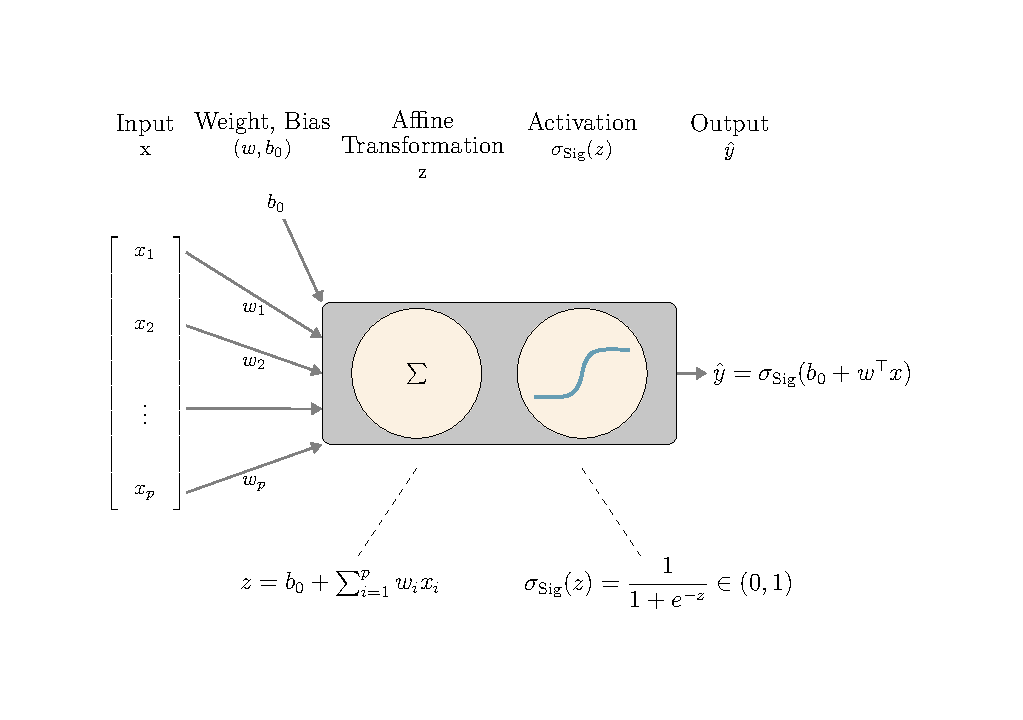
\includegraphics[scale=0.8, trim=0 50 0 50, clip]{figures/logistic_architecture_chapter_book.pdf}
\end{center}
\caption{The sigmoid model represented with neural network terminology as a shallow neural network. Observe that the artificial neuron is composed of an affine transformation using $z = b_0 + w^\top x$ followed by a non-linear activation transformation 
$\sigma_{\text{Sig}}(z)$.} %The gray box represents an artificial neuron composed of an affine transformation to create $z$ and an activation $\sigma_{\text{Sig}}$.}
\label{fig:niceneuron}
\end{figure}

If the model would have not had $\sigma_{\text{Sig}}(~)$, then it would be a {\em linear model}, which we do not cover here. But with it, the $\sigma_{\text{Sig}}(~)$ means a sigmoid function, which takes any scalar input $z$ and produces a probability output $\hat{y}=\sigma_{\text{Sig}}(z)$. The reader can experiment to compute $1/(1+e^{-z})$ with a calculator or spreadsheet for several values of $z$, to see that it always yields numbers that are between $0$ and $1$, and for example with $z=0$ we have $\sigma_{\text{Sig}}(0) = 1/2$. In a deep learning framework, the function, $\sigma_{\text{Sig}}(~)$, is a type of {\em activation function} and the form of \eqref{eq:first-shallow-view} represents an \textit{artificial neuron} which we also present in Figure~\ref{fig:niceneuron}. 


The sigmoid model can be viewed as the simplest non-linear neural network model. %Outside of the context of deep learning, sigmoid model is known as logistic regression and it is also a very popular statistical model \sbmc{[logistic model is a statistical model. This sentence seems to imply differently. How about "
Outside of the context of deep learning, the sigmoid model is very popular in statistics, and known as {\em logistic regression}. This model is suitable for binary classification tasks where \texttt{positive} samples are encoded via $y=1$ and \texttt{negative} samples are encoded via $y=0$.  The output of the model $\hat{y}$ is a number in the continuous range $[0,1]$ indicating the probability that the features vector $x$, matches a \texttt{positive} label. Hence, the higher the value of $\hat{y}$, the more likely it is that the label associated with $x$ is $y=1$. A classifier can be constructed via a \textit{decision rule} based on a threshold $\tau$, with the predicted output being,
%
\begin{equation} %QQQQ - argue/discuss the order
\label{eq:y-hat-tau}
\widehat{\cal Y} = 
\begin{cases}
0~ (\texttt{negative}), & \text{if} \quad  \hat{y} \le \tau \\
1~ (\texttt{positive}), & \text{if} \quad   \hat{y} > \tau.
\end{cases}
\end{equation}
In many cases one selects the threshold at $\tau = 0.5$. \\

\noindent
{\bf Model II}: {\bf The softmax model also known as the multinomial regression model.} Using equations, this model can be described as,

%
\begin{equation}
\label{eq:softeq}
\hat{y}=S_{\text{Softmax}} \big(\overbrace{b+W  x}^{\quad \,\,\, \, \,\, z\, \in \, {\mathbb R}^K}\big),
% \hat{y}=\underbrace{S_{\text{softmax}} \big(\overbrace{b+W  x}^{z\in {\mathbb R}^K}\big)}_{a\in {\mathbb R}^K},
% \end{equation}
%
\qquad
\text{with}
\qquad
%
% \begin{equation}
% \label{eq:softmax-in-mult}
S_{\textrm{Softmax}}(z) = \frac{1}{\sum_{i=1}^{K} e^{z_i}} 
\begin{bmatrix}
e^{z_1} \\
\vdots\\
e^{z_{K}}\\
\end{bmatrix}.
\end{equation}
%
Here like the sigmoid model, the input, denoted $x$, is a vector of dimension $p$, and as before we can denote this as  $x\in {\mathbb R}^p$. However the output, $\hat{y}$ is no longer a single probability, as in Model~I, but is rather a vector of probabilities of length $K$, where the individual probabilities sum up to $1$. The parameters of the model are also different. The parameter $b$ plays the role of $b_0$ from Model~I and is no longer a scalar, but is rather a vector of dimension $K$, and we denote this as $b\in {\mathbb R}^K$. It is called the {\em bias vector}. As for the weights, unlike Model~I where the weights were in a vector, here we have a matrix of weights, or {\em weight matrix}, $W$, of dimensions $K$ and $p$, where $K$ is the number of matrix rows, and $p$ is the number matrix columns. This can be denoted as $W\in {\mathbb R}^{K\times p}$.

Like Model~I in \eqref{eq:first-shallow-view}, here, the operation of the model in \eqref{eq:softeq} denotes an intermediate variable $z$. The difference is that $z$ is a vector of dimension $K$, denoted $z \in {\mathbb R}^K$. Here to construct $z$ we add the vector $b$ to the vector produced by the matrix-vector multiplication $W x$. 
%, a weight matrix of numbers are the parameters of the model. The input $x\in {\mathbb R}^p$ is also a vector, and $b + Wx$ means the matrix-vector multiplication ($Wx$), followed by the vector-vector addition (adding $b$). 
This means that for $i=1,\dots,K$, each scalar, $z_i$ in the vector $z\in {\mathbb R}^K$ is computed as,
%
\begin{equation}
\label{eq:small-zk-log-mult}
z_i = b_i + \sum_{j=1}^p w_{i,j} \, x_j,
\end{equation}
%
where $b_i$ is the $i$-th scalar in the vector $b$ and $w_{i,j}$ is the scalar in the matrix $W$ at row $i$ and column $j$.

Like Model~I, that applies the (non-linear) function $\sigma_{\text{Sig}}(~)$ on the scalar $z$, here with Model~II we apply the function $S_{\textrm{softmax}}(~)$ on the vector $z$. This function is called the {\em softmax} and it converts a vector of dimension $K$ to a different vector of the same dimension $K$, where all elements of the output vector are probabilities, and they sum up to $1$.

\begin{figure}[h]
\begin{center}
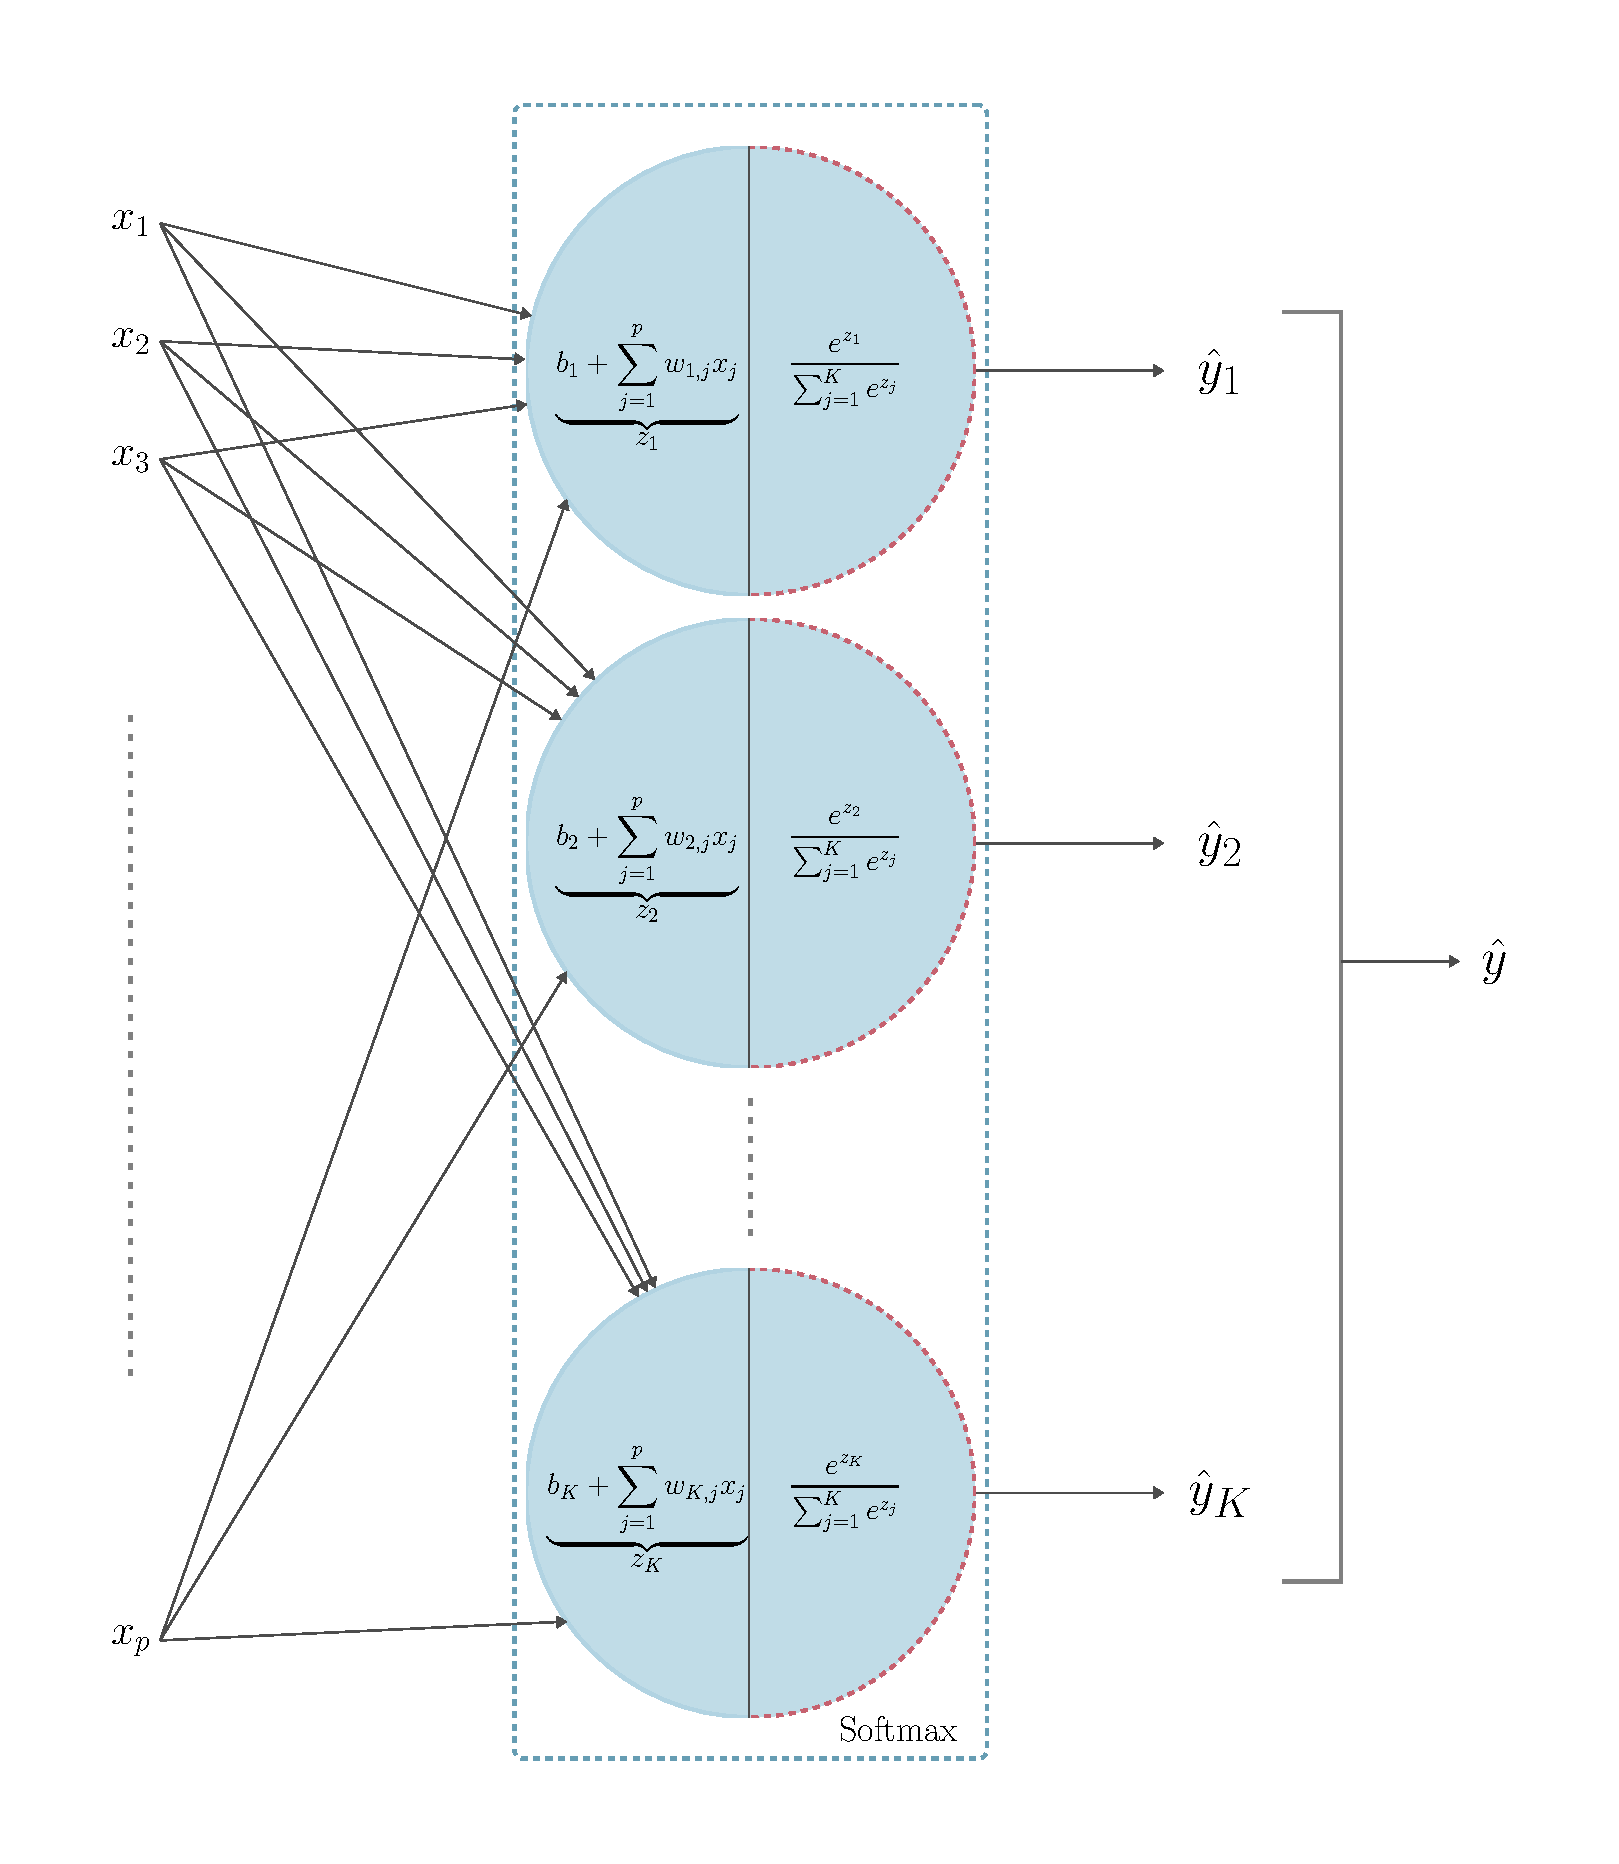
\includegraphics[scale=0.48,trim=50 50 50 50, clip]{figures/figure_softmax.pdf}%softmax_layer.pdf}
\end{center}
\caption{The softmax model as a shallow neural network model with output $\hat{y}$ which is composed of elements $\hat{y}_1, \ldots, \hat{y}_K$,  representing a probability vector. }
\label{fig:shalsoft}
\end{figure}

The form of \eqref{eq:softeq} positions the softmax model as a shallow neural network similarly to the way that the sigmoid model is a shallow neural network. The difference is that the softmax model has vector outputs while the sigmoid model has a scalar output. Figure~\ref{fig:shalsoft} illustrates the softmax model as a neural network. Here each circle can again be viewed as an ``artificial neuron'' however note that the softmax function %\sbmc{[note that the phrase 'activation' is used first time here for this model.]} 
affects all neurons together via the normalization in the denominator of the softmax function $S_{\textrm{softmax}}(~)$. Hence the activation value of each neuron is not independent of the activation values of the other neurons.

The softmax model, also known as the multinomial regression model, is the most popular model for multi-class classification, where the goal is to provide a prediction $\widehat{\cal Y}$ for the label in $\{1,\ldots,K\}$ associated with the input feature vector $x$.  The softmax model produces an output vector, $\hat{y}$, which is a probability vector, and can be used to create a classifier by choosing the class that has the highest probability. Namely,
%
\begin{equation}
\label{eq:argmax-mp}
\widehat{\cal Y}=\underset{k \in\{1, \ldots, K\}}{\operatorname{argmax}} ~\hat{y}_k,
\end{equation}
%
and this means to choose the index $k$ from the set $\{1,\ldots,K\}$, where the entry (probability) $\hat{y}_k$ is highest. 
This approach is called a \textit{maximum a posteriori probability} (MAP) decision rule since it simply chooses $\widehat{\cal Y}$ as the class that is most probable. It is the most common decision rule when using deep learning models for classification. \\

\noindent
{\bf Model III}: {\bf General fully connected neural networks also known as feedforward networks.} Using equations, this model can be described as,
%
\begin{equation}
\label{eq:generalRecursiveModel}
\hat{y}=f^{[L]}(f^{[L-1]}(f^{[L-2]}(\ldots (f^{[1]}(x))\ldots))),
% f_{\mathbf{\theta}}(x)=f_{\mathbb{\theta}^{[L]}}^{[L]}(f_{\mathbb{\theta}^{[L-1]}}^{[L-1]}(\ldots (f_{\mathbb{\theta}^{[1]}}^{[1]}(x))\ldots)),
\end{equation}
%
where each individual function $f^{[\ell]}(~)$ operating on some input $u$, can be  described as,
%
\begin{equation}
\label{eq:dense-layer}
f^{[\ell]}(u) =
S^{[\ell]}(b^{[\ell]} + W^{[\ell]} u),
\qquad
\text{for}
\qquad
\ell = 1,\ldots,L.
\end{equation}
%
Here in \eqref{eq:generalRecursiveModel} we see composition of functions, where first the function $f^{[1]}(~)$ is applied to the input $x$, and then the function $f^{[2]}(~)$ is applied on the output of $f^{[1]}(x)$, and then $f^{[3]}(~)$ is applied on the output of $f^{[2]}(f^{[1]}(x))$, and so fourth until the last function $f^{[L]}(~)$ is applied on what was computed prior. Each such function application is the operation of a {\em layer} in a deep neural network. 

Different types of neural networks have different types of layers, and in the simplest case of feedforward fully connected neural networks, \eqref{eq:dense-layer} describes the operation of layer~$\ell$. Observe that \eqref{eq:dense-layer} is somewhat similar to the left side of \eqref{eq:softeq}. In the case of \eqref{eq:dense-layer}, we have that $S^{[\ell]}(~)$ is some vector activation function, while in the case of \eqref{eq:softeq} there is only a single layer (and hence $\ell$ is absent) and the activation function is the softmax function.  

\begin{figure}[h!] 
\begin{center}
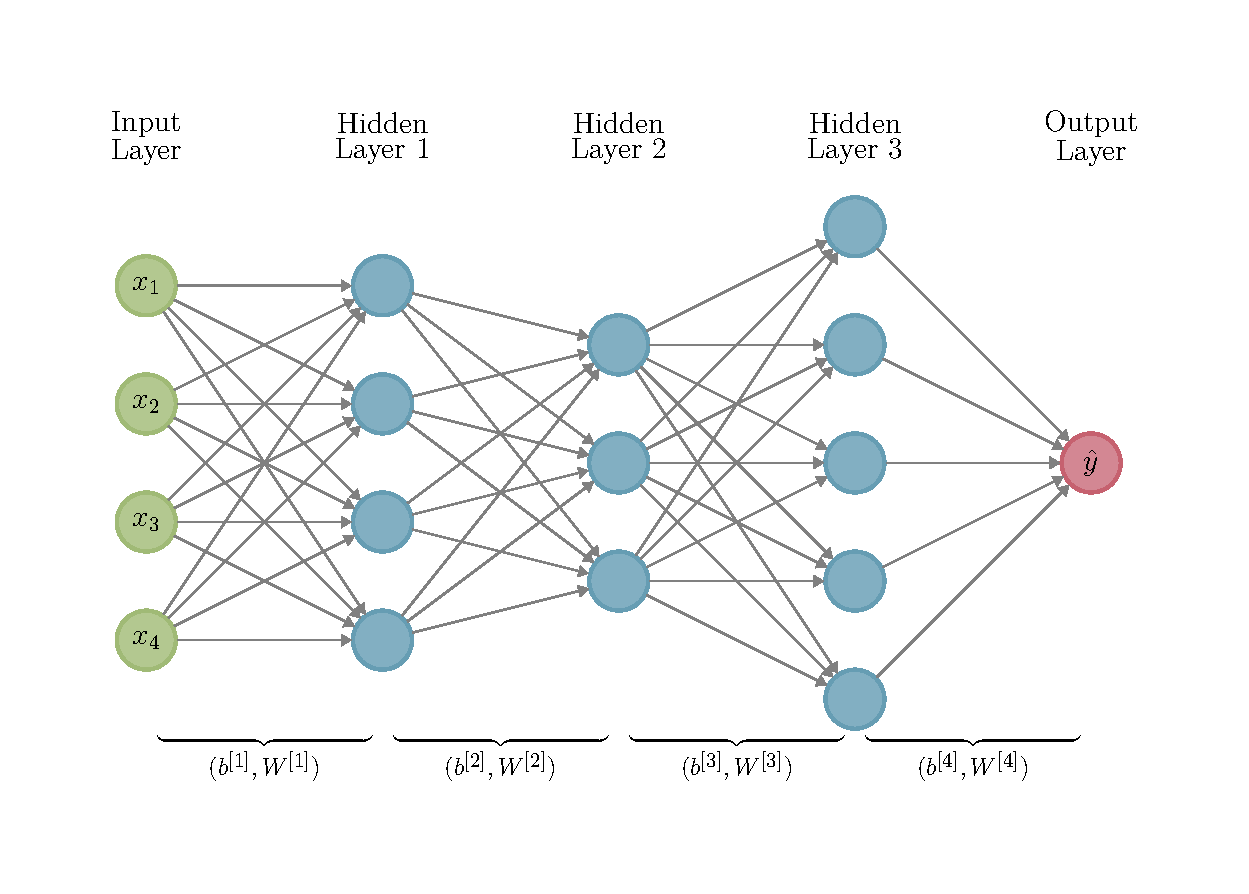
\includegraphics[scale=0.7,trim=0 40 0 50, clip]{figures/deep_neural_network1.pdf}
 \caption{A fully connected feedforward deep neural network with multiple hidden layers. The input to the network is the vector $x = (x_1, x_2, x_3, x_4)$ and in this case the output is the scalar~$\hat{y}$. For this particular example the dimensions of $W^{[1]}$ are $4\times 4$, $W^{[2]}$ is $3 \times 4$, $W^{[3]}$ is $5 \times 3$, and $W^{[4]}$ is $1 \times 5$. The bias vectors are of dimension $4$ for $b^{[1]}$, $3$ for $b^{[2]}$, $5$ for $b^{[3]}$, and $1$ (a scalar) for $b^{[4]}$.
 }
    \label{FFNN}
\end{center}
\end{figure}

The parameters of each layer $\ell$ are also similar to Model~II (which only has a single layer). Here with Model~III, each layer has a {\em bias vector} $b^{[\ell]}$ and a {\em weight matrix} $W^{[\ell]}$. The dimensions of these vectors and matrices are specific to the architecture of the network, and we fill in these details in Section~\ref{sec:putting-bits-together}. At this point, let us appreciate that Model~III is more complex. For one thing, it has the rich set of parameters $(b^{[1]}, W^{[1]}), \ldots, (b^{[L]}, W^{[L]})$ which can easily involve hundreds of thousands, millions, or billions of individual scalar parameters.  With so many parameters organized in layers, it is generally much more expressive and can capture complex relationships in data. Figure~\ref{FFNN} presents a schematic of such a deep neural network.

%%%%%%%%%%%%%%%%%%%%%%%%%%%%%%%%%%%%%%%%
%%%%%%%%%%%%%%%%%%%%%%%%%%%%%%%%%%%%%%%%
%%%%%%%%%%%%%%%%%%%%%%%%%%%%%%%%%%%%%%%%
\section{Data Standardization and Recalling Summation Notation}
\label{sec:summation}

Raw data often requires \textit{preprocessing} before it can be used in a deep learning model. One such form of preprocessing is \textit{standardization of the data}, also sometimes called \textit{normalization of the data}. This involves subtraction of the mean and division by the standard deviation. Let us describe how this is done here and in the process review summation notation which is needed for other purposes also.

Assume that our data is $x^{(1)}, \ldots, x^{(n)}$ where each $x^{(i)}$ is some sample which is a list or vector of length $p$. We can also denote $x_j^{(i)}$ as the $j$-th element (or coordinate) of the $i$-th data sample. Hence we can think of the data as an $n$ by $p$ table, or matrix, where each row is a sample, and each column is a specific part of that sample, sometimes called a {\em feature}.

For instance, consider a dataset consisting of medical measurements for patients, where each patient's data includes their age, blood pressure, and cholesterol level. This means that $p=3$. As an example, this data may look as follows:
%
\[
\begin{array}{c}
% \hspace{4.4cm}
\text{Age} \quad \text{Blood Pressure} \quad \text{Cholesterol Level} \\
\end{array}
\]
\begin{equation}
\label{eq:data-table}
% \text{Raw Medical Data: }
\left[ \begin{array}{ccc}
50 & 120 & 200 \\
35 & 130 & 220 \\
\vdots & \vdots & \vdots \\
\vdots & \vdots & \vdots \\
\phantom{\text{Age}} & \phantom{\text{Blood Pressure}} & \phantom{\text{Cholesterol Level}}\\
\vdots & \vdots & \vdots \\
\vdots & \vdots & \vdots \\
45 & 125 & 190 \\
\end{array} \right]
\end{equation}
%
The number of observations $n$ is the number of rows in the table.
In this example, the second observation in the second row, $x^{(2)}= (35,130,220)$, corresponds to the information of the second patient. Similarly, $x_3^{(1)} = 200$ is the cholesterol level for the first patient. 

You can now take all the sample values for some feature $j$, and denote them as $x_j^{(1)}, \ldots, x_j^{(n)}$. This would be one column of the data.  
Now for this column we can compute the \textit{sample mean} and \textit{sample variance} respectively as,
%
\begin{equation}
\label{eq:stats-mean-var}
\overline{x}_j = \frac{1}{n} \sum_{i=1}^n x_j^{(i)},
\qquad
s^2_j = \frac{1}{n} \sum_{i=1}^n (x_j^{(i)} - \overline{x}_j)^2.
\end{equation}
%
Further, the \textit{sample standard deviation} is the square root of the sample variance and is denoted via $s_j$. Note that in statistics one sometimes divides by $n-1$ instead of $n$ for the sample variance, but this is a detail we will skip here. Our purpose in presenting \eqref{eq:stats-mean-var} is also that we review summation notation (with $\Sigma$, i.e., Sigma).

To review summation notation, consider an expression where we have some list of $4$ numbers, $h^{(1)}, h^{(2)}, h^{(3)}, h^{(4)}$ with $h^{(1)} = 2$, $h^{(2)} = 4$, $h^{(3)} = 0$, and $h^{(4)} = 10$. Then this arbitrary expression,
%
\begin{equation}
\label{eq:4-summation}
\sum_{i=1}^4 h^{(i)},
\end{equation}
%
is just shorthand for $h^{(1)} +h^{(2)} +h^{(3)} +h^{(4)}$. It thus equals $16$ in this example. One can think of the variable $i$ as ``running'' from $i=1$ all the way up to $i=4$. We could have also used $j$ instead of $i$ or any other variable name. One could have obviously had more complicated expressions with summation notation, such as for example,
%
\begin{equation}
\label{eq:4-summation-advc}
\sum_{i=1}^4 (h^{(i)} +h^{(5-i)} - 11)^2,
\end{equation}
%
which the reader can verify equals $100$.

Now in \eqref{eq:stats-mean-var} we first use summation notation in the most basic manner to compute the sample mean for feature $j$ which we denote as $\overline{x}_j$. This is then used to compute the sample variance for that feature which we denote as $s_j^2$. Then the sample standard deviation, $s_j$, is just the square root of $s_j^2$.

With our data, once we have the sample mean and sample standard deviation for each feature, we may standardize the data samples of each feature $j=1,\ldots,p$ and each observation $i=1,\ldots,n$ to obtain \textit{standardized samples},
%
\begin{equation}
\label{eq:ref-stand-z}
\tilde{x}^{(i)}_j = \frac{x^{(i)}_j - \overline{x}_j}{s_j}.
\end{equation}
%
These standardized observations can also be placed in an $n$ by $p$ table just like the original data. Now the standardized data for feature $j$, $\tilde{x}_j^{(1)}, \ldots, \tilde{x}_j^{(n)}$, has a sample mean of exactly~$0$ and a sample standard deviation of exactly~$1$. In the case the data samples of the feature are distributed according to a normal (Gaussian) distribution then most standardized samples would lie in the range $[-3,3]$. Even if the data is not normally distributed, the standardized samples will still lie in the vicinity of this range and are centered about $0$.

Such standardization is useful as it places the dynamic range of the model inputs on a uniform scale and thus improves the numerical stability of algorithms. It also allows us to use similar models for different datasets that may, without standardization, have completely different dynamic ranges. It is one of many tricks of the trade when dealing with data for deep learning. We also chose to present it here as a basic review of summation notation.

%%%%%%%%%%%%%%%%%%%%%%%%%%%%%%%%%%%%%%%%
%%%%%%%%%%%%%%%%%%%%%%%%%%%%%%%%%%%%%%%%
%%%%%%%%%%%%%%%%%%%%%%%%%%%%%%%%%%%%%%%%
\section{From Basic Sets to Functions}
\label{sec:sets-and-functions}

Almost all of mathematics starts with the notion of a {\em set}. Formally, a set is an unordered collection of unique items, and sets are typically denoted like $\{7,\, 2.5,\, \texttt{hello}\}$, where the curly braces, $\{\}$, indicate that this is a set. In this particular example the set is composed of the number $7$, the number $2.5$, and the text \texttt{hello}. Like anything in mathematics, we can name sets, and we could have also written ${\cal A} = \{7,\, 2.5,\, \texttt{hello}\}$ to name this set as  ${\cal A}$.

Each of $7$, $2.5$, and \texttt{hello} are {\em elements} of the set ${\cal A}$. And we can write $7 \in {\cal A}$, to imply that $7$ is an element of ${\cal A}$, and similarly with $2.5$ and \texttt{hello}. This ``in'' symbol, $\in$, is useful for statements such as: ``for all $u \in {\cal A}$ do something with $u$''. This means, ``do something with $7$, and do something with $2.5$, and do something with \texttt{hello}''. We can also say that $4 \notin {\cal A}$, because $4$ is not an element of ${\cal A}$. That is $\not\in$ is ``not in'' with the slash across the $\in$ symbol. 

Sometimes we define sets in less explicit ways. For example ${\cal B} = \{0,2,4,6,\ldots,20\}$ is the set of all even numbers between $0$ and $20$ including $0$ and $20$. And this is clear to us even though we did not write out every element of ${\cal B}$. We can also use sets within summation notation. For example, 
%
\begin{equation}
%\label{eq:4-summation-set}
\sum_{u \in {\cal B}} \sqrt{u},
\end{equation}
%
implies summing up all of the square roots of the elements of the set ${\cal B}$ (as the reader may verify, the result is approximately $31.77$). Note  that our previous way of using summation notation can also be written in terms of sets. For example, the summation in \eqref{eq:4-summation} can be written as,
%
\begin{equation}
%\label{eq:4-summation-set}
\sum_{i \in \{1,2,3,4\}} h^{(i)},
\end{equation}
%
as this shows that the variable $i$ runs on each element of the set $\{1,2,3,4\}$. 

One very important set is the set of real numbers, denoted ${\mathbb R}$. Unlike the example sets ${\cal A}$, ${\cal B}$, or $\{1,2,3,4\}$ which only have a finite number of elements, the set ${\mathbb R}$ has every number on the real number line and is hence not a finite set. We again can speak about elements of ${\mathbb R}$. So for example it is true that $7 \in {\mathbb R}$,  and it is also true that $\texttt{hello} \not\in {\mathbb R}$. When we consider the parameters of Model~I in \eqref{eq:first-shallow-view}, we can write $b_0 \in {\mathbb R}$ to signify that $b_0$ is a real number.

We can also denote the set of real numbers as $(-\infty, \infty)$ implying that it is the interval of all numbers that are greater than $-\infty$ and less than $\infty$, and this means all real numbers. There are other sets that we can denote in a similar way, for example $[-1,1]$ is the set of all numbers greater than or equal to $-1$ and less than or equal to $1$. Another option is the set $(0,\infty)$ which means the set of all positive numbers (greater than $0$). The set $[0,1]$ is the set of all real number between $0$ and $1$ inclusive, and this is basically all numbers that can describe a probability. A related set $(0,1)$ contains all the numbers between $0$ and $1$ but without the boundaries $0$ and $1$.

One can study and discuss sets much further, and in a more formal manner, or even in very formal means that relate to mathematical logic. But our purpose here is simply to introduce minimal notation. For this, we present a few more sets when dealing with vectors and matrices in the sections below. But first, at this point, with our basic understanding of sets, we are ready to discuss the notion of a {\em function}. 

Put simply, a function is an operation that transforms elements from one set to elements of another set. We can for example denote our function as $f$ and think that it operates on inputs from the set ${\cal A} = \{7,\, 2.5,\, \texttt{hello}\}$ and gives us outputs from the set of real numbers~${\mathbb R}$. Formally this can be denoted as,
%
\begin{equation}
\label{eq:some-func}
f: {\cal A} \to {\mathbb R},
\end{equation}
%
and this notation tells us that all of the possible inputs to the function $f(~)$ are the elements of~${\cal A}$. It further says that the outputs must be elements of the real numbers ${\mathbb R}$. This declaration of the function via \eqref{eq:some-func} says that for every $u \in A$ we should have an answer of what the function gives, and we denote this as $f(u)$. Note that we sometimes write $f(\cdot)$ to indicate the function where ``$\cdot$'' just stands for the place where the argument $u$ should appear. 

A declaration such as \eqref{eq:some-func} does not define how the function works. To do so, we must be more explicit either with a formula, or an algorithm, or a lookup table. In this example, since the input set has a small number of heterogeneous elements, let us specify the function via a lookup table approach. In particular we can state, $f(7) = 3.4$, $f(2.5) = -2.1$, and $f(\texttt{hello}) = 20.3$. This would then specify exactly what the function $f(~)$ does for every $u \in {\cal A}$. 

In other cases, we can specify how the function works with a formula. This is often common for functions $f: {\mathbb R} \to {\mathbb R}$. An arbitrary example of such a function from ${\mathbb R}$ to ${\mathbb R}$ is,
%
\begin{equation}
\label{eq:arb-func-r-to-r}
f(u) = 3\cos(e^{u-2}).
\end{equation}
%
The reader would have seen plots previously where such a function, or others, are plotted where on the horizontal axis we plot $u$ and on the vertical axis we plot $3\cos(e^{u-2})$. Importantly, for every $u \in {\mathbb R}$ we have a specific $y = f(u)$, and the plot is a connection of the points $(u,f(u))$ on the plane, essentially for every $u \in {\mathbb R}$ (or realistically on some smaller set which defines the domain of the plot). Also note that in this case the function \eqref{eq:arb-func-r-to-r} is {\em composed} of other operations and functions such as the cosine function and the exponentiation function. Indeed function composition is a very common operation where outputs of one function are used as inputs of another. An example is with Model~III as in \eqref{eq:generalRecursiveModel} where we have $L-1$ function compositions and each function represents the operation of a layer of neural network.

In deep learning we use functions in multiple ways. One way is for constructing models such as I -- III. Another way is for specifying the whole model as a function. A third way is for construction of loss functions. Let us now highlight such uses.

First in terms of construction of models, as we can see for Model~I in \eqref{eq:first-shallow-view},  we define the {\em sigmoid function} 
%
\begin{equation}
\label{eq:sig-as-func}
\sigma_{\text{Sig}}: {\mathbb R} \to [0,1].
\end{equation}
%
This function takes any real valued scalar as input, denoted as $z$ in \eqref{eq:first-shallow-view}, and the output is a number in the range $[0,1]$. Note that for this sigmoid function we have a formula, $1/(1+e^{-z})$, which exactly describes how to compute $\sigma_{\text{Sig}}(z)$. A schematic plot of this function is inside the right circle in Figure~\ref{fig:niceneuron}.


Further, for Model~II in \eqref{eq:softeq} we have the softmax function, $S_{\textrm{Softmax}}(z)$ as a building block. This function can be declared as,
%
\begin{equation}
\label{eq:softmax-as-func}
S_{\textrm{Softmax}}: {\mathbb R}^K \to {\mathbb R}^K,
\end{equation}
%
since it takes $K$-dimensional vectors as inputs and returns $K$-dimensional vectors as outputs. We describe it further in the next section after we discuss vectors. Similarly, for Model~III, we have activation functions for deep feedforward neural networks, $S^{[\ell]}(\cdot)$. We discuss such activation functions in Section~\ref{sec:putting-bits-together}. 

Now a different use of functions for the neural network models I, II, and III is that the whole model is a function that converts some input~$x$ to an output~$\hat{y}$. In terms of all three models, I -- III, the input $x$ is a $p$-dimensional list of numbers, or vector, a notion further discussed in the next section. For now, let us agree that this set is denoted as~${\mathbb R}^p$. The output is either a scalar value (an element of ${\mathbb R}$ or an element of $[0,1]$) or a vector which is an element of ${\mathbb R}^K$ (a vector or list of $K$ numbers). In particular, here are the functions described by these models.

For Model~I, yielding a probability output we can declare the function of the model as,
%
\begin{equation}
\label{eq:model-I-f}
f_{(b_0,w)}: {\mathbb R}^p \to [0,1].
\end{equation}
%
The representation in \eqref{eq:model-I-f} then tells us that inputs to the model are $x \in {\mathbb R}^p$ and outputs are going to be $\hat{y} \in [0,1]$. Now notice that we also decorate the function name $f$ with a subscript $(b_0,w)$, and this subscript signifies the parameters of the model. In particular, when we train a deep learning model such as this, we find suitable values of the parameters $b_0$ and $w$ for the data. These parameters then exactly dictate the specifics of our model function $f_{(b_0,w)}(~)$. The way the function actually works was already specified in \eqref{eq:first-shallow-view}. However, some specifics of that presentation, such as the inner product $w^\top x$, are explained in the next section. In Figure~\ref{fig:breast-log-curves} we see two example plots for two different instances of \eqref{eq:model-I-f} where each time we plot $\hat{y} = f_{(b_0,w)}(x)$. In (a) we see a case with $p=1$, and we also see data points for which the function was fit. In (b) we see a case with $p=2$, this time without the data points. 

\begin{figure}[h!] 
  \begin{subfigure}[b]{0.45\linewidth}
    \centering
    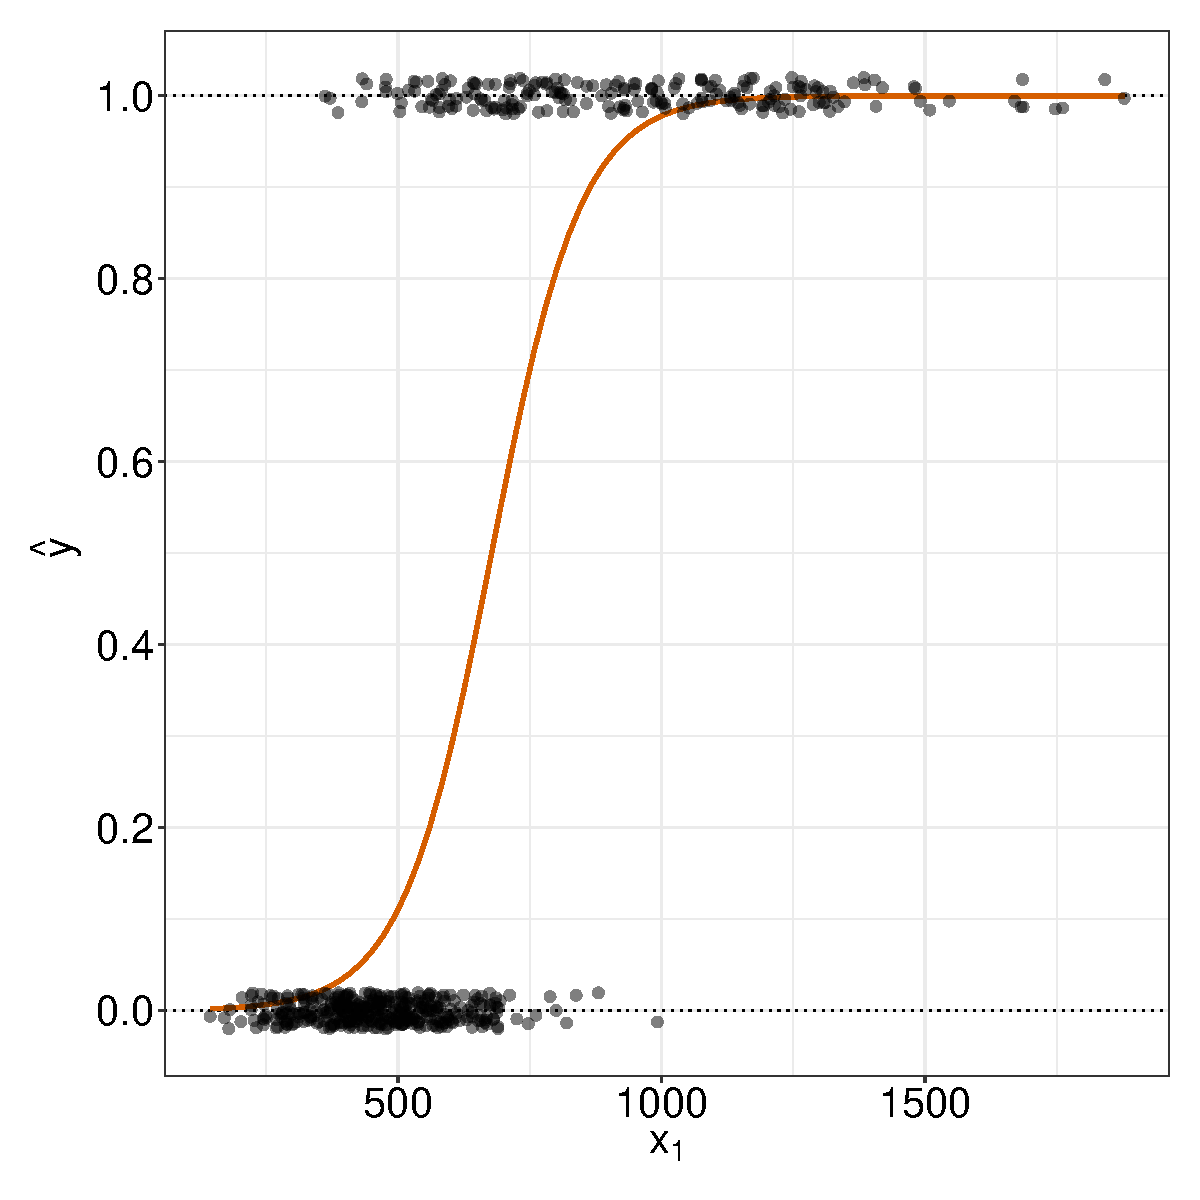
\includegraphics[width=0.95\linewidth, height=1.2\textwidth]{figures/Figure-LINK-UNIVARIATE-chapt.pdf} %trim=0 0 0 0, clip
    \caption{} 
%    \vspace{2ex}
  \end{subfigure}%% 
~
  \begin{subfigure}[b]{0.45\linewidth}
   % \centering
    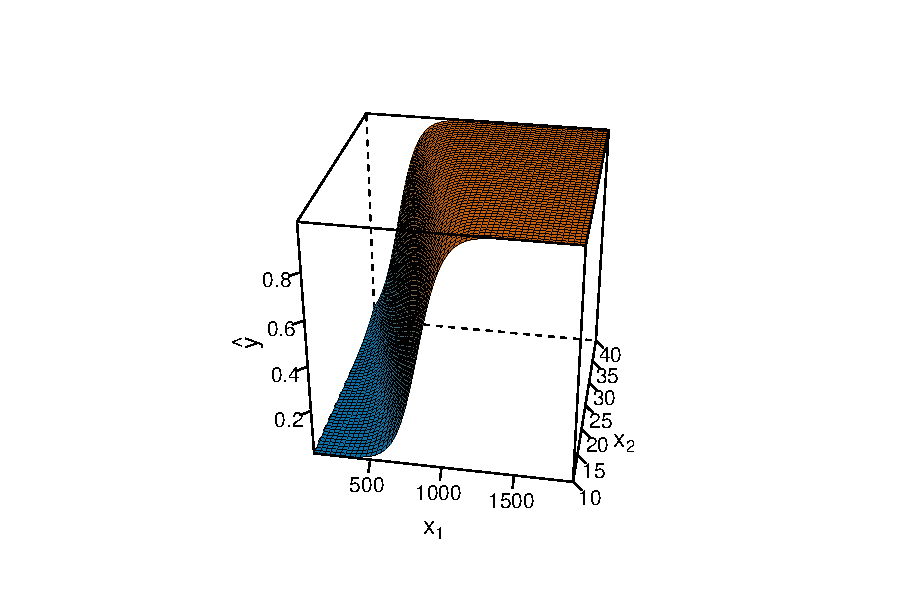
\includegraphics[width=0.99\linewidth, angle=-5, trim={0 10 30 10}]{figures/logistic-2-features-cropped.pdf} %,trim=100 0 0 0, clip
    \caption{} 
%    \vspace{2ex}
  \end{subfigure} 
    \caption{Probability output using Model I. % prediction fitto the Wisconsin breast cancer dataset. 
    (a) A $p=1$ model with one feature. % \texttt{area\_mean} ($x_1$)and a confidence band. 
    (b) A $p=2$ model based on two features. %5\texttt{area\_mean} ($x_1$) and \texttt{texture\_mean} ($x_2$).
    }
    \label{fig:breast-log-curves}
\end{figure}


For Model~II, the function of the model can be specified as,
%
\begin{equation}
\label{eq:model-II-f}
f_{(b,W)}: {\mathbb R}^p \to {\mathbb R}^K,
\end{equation}
%
and in particular the output in this case is a $K$-dimensional vector. The parameters of the model are $(b,W)$, and more details about how the model operates are in the sequel.

For Model~III, we leave the specification of the type of output open. In some cases it can be a single probability value, so we may specify the output as a value in the set $[0,1]$. In other cases it can be a single real number, as one typically has in {\em regression problems}. Thus the output can be specified as a value in ${\mathbb R}$. We can also use Model~III for multi-class classification like Model~II and then the output is a vector as with Model~II, so the output is a value in ${\mathbb R}^K$ (also sometimes denoted ${\mathbb R}^q$). One way to write this is,
%
\begin{equation}
\label{eq:model-III-f}
f_{(b^{[1]}, W^{[1]}), \ldots, (b^{[L]}, W^{[L]})}: {\mathbb R}^p \to {\cal O},
\qquad
\text{where}
~{\cal O}~
\text{is}~[0,1],~\text{or}~
{\mathbb R},~\text{or}~{\mathbb R}^q.
\end{equation}
%
In all these scenarios of Model~III, the input is similar to the other two models, but for the output type there are several options. Observe also the rich set of parameters that the model has, namely, $(b^{[1]}, W^{[1]}), \ldots, (b^{[L]}, W^{[L]})$.

Another use of functions in deep learning is {\em loss functions}. In general when we train a model we are given a fixed dataset and wish to find the best set of parameters such that the model fits the data. For example with Model~II we would seek the best possible vector $b$ and matrix $W$ that we can find to match the data.  The way that this ``bestness'' is quantified is via a function that we artificially construct for the model. Unlike the model functions \eqref{eq:model-I-f}, \eqref{eq:model-II-f}, and \eqref{eq:model-III-f} which operate on the input $x$, the loss function is a function of the parameters, and the training data is fixed for this function and determines its shape.


\begin{figure}[h!] 
  \begin{subfigure}[b]{0.5\linewidth}
    \centering
    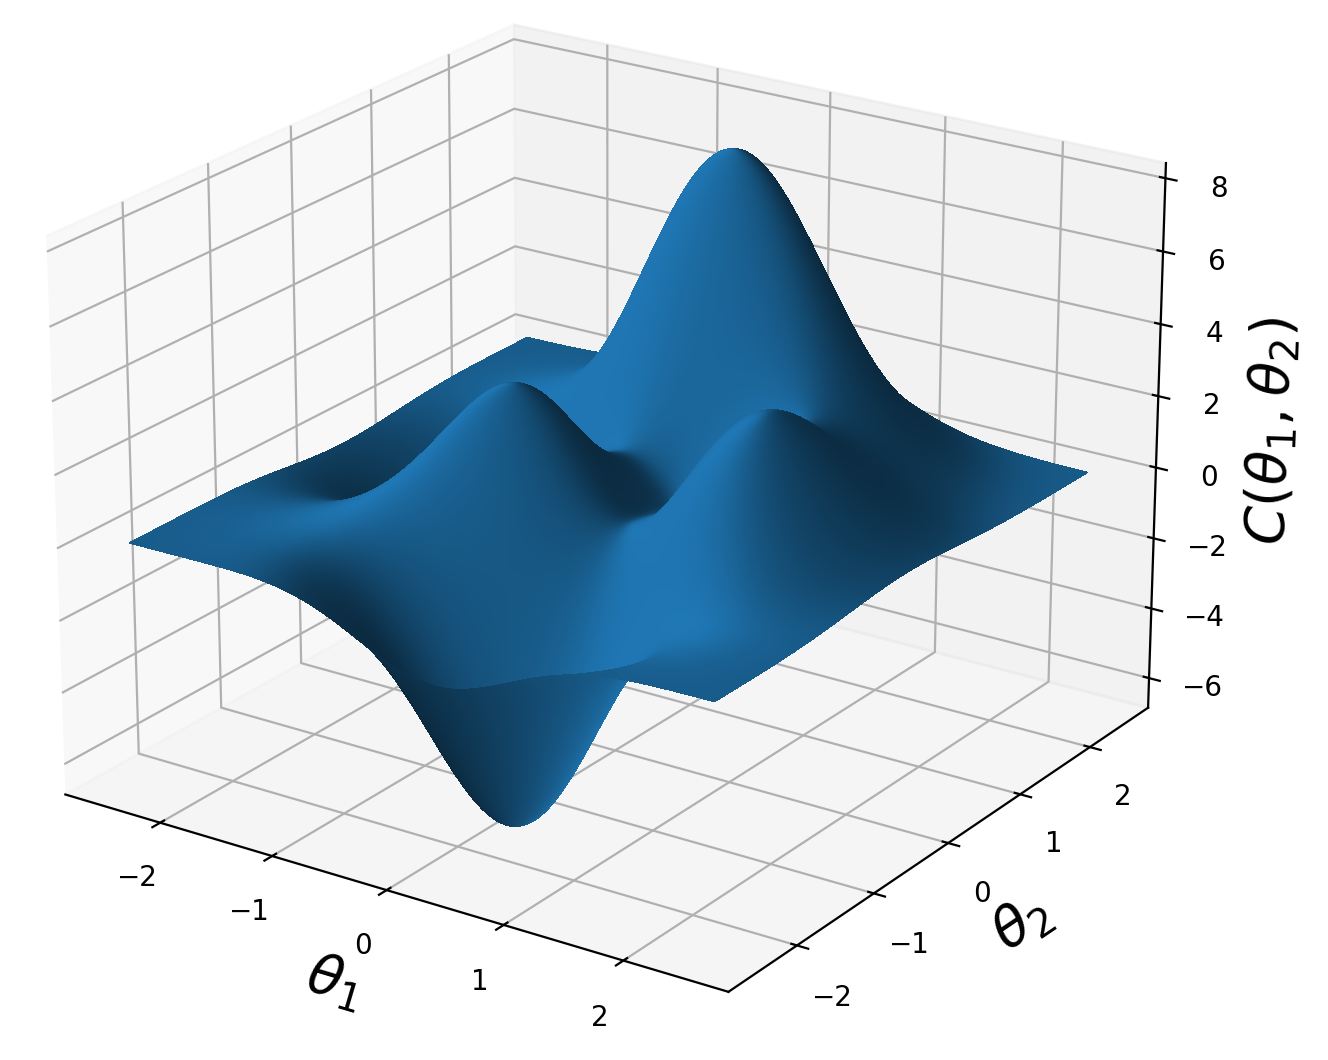
\includegraphics[width=0.87\linewidth, trim=30 30 30 30]{figures/Non-convex-3d.png}
    \caption{} 
    \vspace{2ex}
  \end{subfigure}%% 
  \begin{subfigure}[b]{0.5\linewidth}
    \centering
    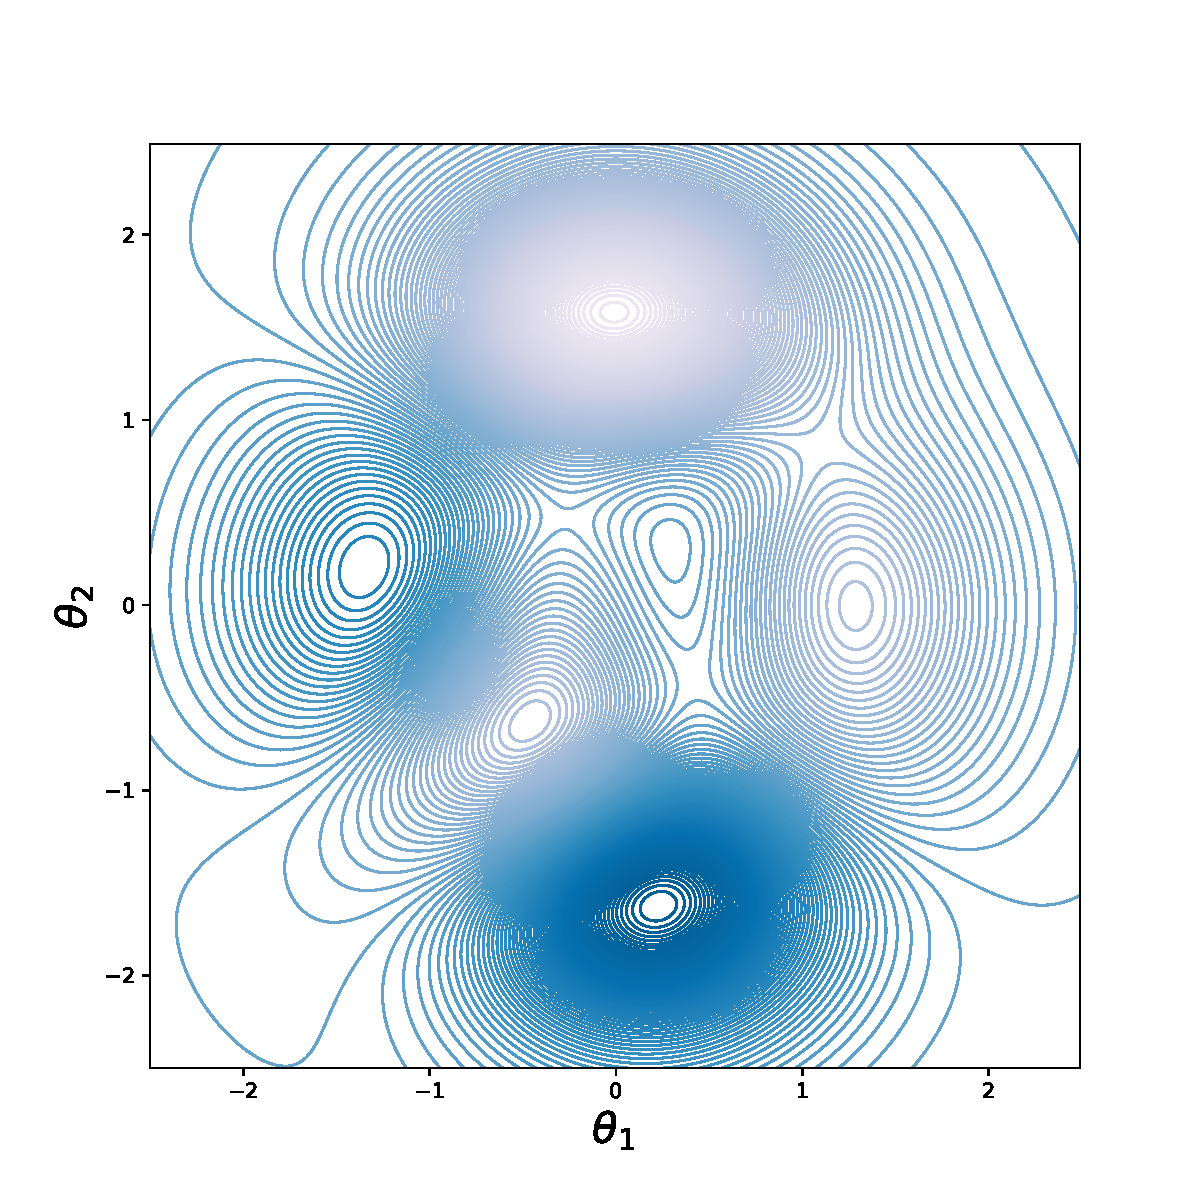
\includegraphics[width=0.77\linewidth, trim=30 30 30 30]{figures/Non-convex-contour.pdf}
    \caption{} 
    \vspace{2ex}
  \end{subfigure} 
    \caption{An example plot of an hypothetical loss function (also known as loss landscape) when there are two parameters. (a) A 3D surface plot where we see that the function has multiple valleys (local minima). (b) The same function can be plotted using a contour plot, where each line along a contour maintains the same value of the loss function (like a topographical map).}
    \label{fig:GD-LR-SR}
\end{figure}

Now since each type of model has a different set of possible parameters, it is common to just call all the parameters $\theta$. In this case $\theta$ can signify $(b_0,w)$ for Model~I, $(b, W)$ for Model~II, and so fourth. We further call the set of all possible parameters $\Theta$ (and the specific form of this set depends on the model type that we use). The loss function, can then be written as,
%
\begin{equation}
C_{\textrm{Data}}: \Theta \to {\mathbb R},
\end{equation}
%
where the subscript, ``Data'', reminds us that the function's actual form depends on the training data that we have. Now in many cases, each $\theta \in \Theta$ contains many parameters (numbers). Especially for example with Model~III, where one can quickly get millions of parameters in a deep neural network.



The act of learning the parameters, or training the model, is the act of finding some $\theta \in \Theta$ where $C_{\textrm{Data}}(\theta)$ is as low as possible or close to the lowest value. This is an optimization problem where we try to minimize the loss $C_{\textrm{Data}}(~)$.

Now when the number of parameters in each $\theta$ is $1$ or $2$, it is possible to plot the loss function and then visualize the minimization of the loss. Such plots are typically not done for operational purposes but rather for pedagogic purposes. In particular, the case of $\theta$ being composed of two numbers $\theta_1$ and $\theta_2$ is easy to plot, and such plots allow us to also think about the techniques and challenges of minimizing loss in general. In Figure~\ref{fig:GD-LR-SR} we present a plot of such an hypothetical loss function.

%%%%%%%%%%%%%%%%%%%%%%%%%%%%%%%%%%%%%%%%
%%%%%%%%%%%%%%%%%%%%%%%%%%%%%%%%%%%%%%%%
%%%%%%%%%%%%%%%%%%%%%%%%%%%%%%%%%%%%%%%%
\section{Vectors}
\label{sec:vectors}

Now that we understand the basics of sets and functions, let us advance to the concept of a {\em vector}. As already seen in Models I -- III, the input $x$ to the model is a vector. This is a list of numbers which encodes some form of input data. Vectors can also appear as outputs. Specifically, in Model~II, and in some variants of Model~III, the output, $\hat{y}$ is also a vector. For example, with Model~II and $K=4$ we may have an output vector such as,
%
\begin{equation}
\label{eq:example-y-hat}
\hat{y} =
\begin{bmatrix}
0.14 \\
0.02\\
0.65 \\
0.19\\
\end{bmatrix},
\end{equation}
%
which in this case marks the probabilities of the four classes of classification (observe that in this example the numbers are non-negative and sum up to $1$). When we have a vector, we often relate to the individual components via a subscript, so that for example $\hat{y}_1 = 0.14$. In this example vector, we see that $\hat{y}_3 = 0.65$ is the highest probability, so if this is a classification output, then we would choose $\widehat{\cal Y} = 3$ as our classification choice using \eqref{eq:argmax-mp}.

The set of vectors of length or {\em dimension $n$} is denoted as ${\mathbb R}^n$. So for example, for the vector $\hat{y}$ of \eqref{eq:example-y-hat} we can write $\hat{y} \in {\mathbb R}^4$. Note that in different texts, vectors are denoted differently. For us, let us also write the same vector as $\hat{y} = (0.14,\, 0.02,\, 0.65,\, 0.19)$. The use of the round brackets, $(~)$, is sometimes associated with the term {\em tuple}, which is similar to a vector and for our purposes may mean the same thing. Also note that the way we wrote the vector in \eqref{eq:example-y-hat} is as a {\em column vector} (the vector is standing up). This way of writing is especially relevant when we do matrix-vector multiplication in the next section. Similarly, one may write $\hat{y} = [ 0.14~~ 0.02~~0.65~~0.19]^\top$, where in this case we first wrote a {\em row vector} $[ 0.14~~ 0.02~~ 0.65~~ 0.19]$ and then applied {\em transpose} to it using the $\top$ symbol in superscript. For vectors, such transposition simply converts them from column to row, and vice-versa. More on this operation appears below in the context of matrices.

For a data scientist and a machine learner, vectors are first and foremost considered as lists of numbers. But in fields such as physics, or applied mathematics, vectors also typically describe directions and magnitudes. This is very apparent in two dimensional spaces or three dimensional spaces. When we discuss gradient vectors in Section~\ref{sec:gradient} below, we also consider vectors as directions in space. But for now first let us think of vectors as lists of numbers, exactly playing the role of inputs, outputs, parameters, and intermediate computations in models such as our example models I -- III.

Note that single numbers, known as {\em scalars}, can be compared in the sense that one is greater than the other (as long as they are {\em real numbers} and not {\em complex numbers} which we do not often use in deep learning). For example we know that $2.4$ is greater than $-8.3$, denoted $-8.3 < 2.4$. If we treat all the scalar real numbers as the set ${\mathbb R}$, then we say there is an order on ${\mathbb R}$, because for every $u \in {\mathbb R}$ and $v \in {\mathbb R}$ one can determine if $u < v$ is true or false. With vectors, unlike scalars, there is not such an obvious order. 

While there is not an obvious universal way to order vectors, we can associate scalars (numbers) with the distances between two vectors, as well as with the length of individual vectors, and these scalars can then be used for ordering and other purposes. One of the most basic ways to do this is the {\em inner product} which for a vector $u \in {\mathbb R}^n$ and a vector $v \in {\mathbb R}^n$, is written as $u^\top v$ or sometimes as $u \cdot v$. The inner product is computed as,
%
\begin{equation}
\label{eq:inner product}
u^\top v = \sum_{i=1}^n u_i v_i = u_1 v_1 + u_2 v_2 + \ldots + u_n v_n.
\end{equation}
%
Hence it is a summation of the products of the individual entries of the vectors. So for example, as the reader may verify for $u=(2,\, 0, \, -3)$ and $v=(1,\, -12.5, \, 2)$, the inner product is $u^\top v = -4$. When the inner product is near $0$ it means that the vectors are quite different, whereas when the inner product is far from $0$ (either positive or negative) it means that the vectors are similar. When the inner product is exactly $0$ we say that the vectors are {\em orthogonal}. In a geometric representation this means the vectors are perpendicular. We do not dive into such a representation of vectors, and instead the interested reader can visit a text such as \cite{boyd2018introduction} for further reading.

If we now return to Model~I and revisit \eqref{eq:first-shallow-view} and \eqref{eq:smallz-only-log-mult}, then we can observe the inner product $w^\top x$ in these equations. Here $w$ is the vector of weight parameters of the model and $x$ is the model input.

One can also compute the {\em norm}  of a vector $u \in {\mathbb R}^n$, denoted as $\| u\|$ and computed as the square root of the inner product of the vector with itself (this is sometimes called the L2 norm or the Euclidean norm). That is,
%
\begin{equation}
\label{eq:norm-vec}
\| u \| = \sqrt{u^\top u} = \sqrt{\sum_{i=1}^n u_i^2}.
\end{equation}
%
For example for $u=(2, \, 0,\, -3)$ as before, $\| u \| = \sqrt{13} \approx 3.6$. The norm of a vector is always a non-negative number and is exactly $0$ if and only if all the entries of the vector are $0$, and otherwise it is strictly positive. So while we cannot order vectors in a unique manner, we can order vectors based on their norm which is a number  that summarizes their magnitude. 

Now that we have norm, we can also consider a scaled version of the inner product which is called the {\em cosine of the angle} between two vectors. For $u \in {\mathbb R}^n$ and $v \in {\mathbb R}^n$, as long as neither of these vectors is all $0$, this is computed as,
%
\begin{equation}
\label{eq:cosine-angle-vec}
\textrm{Cosine of the angle between $u$ and $v$} = \frac{u^\top v}{\|u \|\, \|v\|} = \frac{\sum_{i=1}^n u_i v_i}{\sqrt{\sum_{i=1}^n u_i^2} \, \sqrt{\sum_{i=1}^n v_i^2 }}.
\end{equation}
%
So for example for the $u$ and $v$ examples above, the cosine of the angle is about $-0.087$. The cosine of the angle is always between $-1$ and $1$ and the closer it is to $0$ the less similar the vectors are in some sense. It is exactly $0$ if the vectors are orthogonal.

All of the above definitions and computations of vectors are very common to use in deep learning. One more thing that we do is arithmetic with vectors. The most basic operation is to take a scalar (a single number) and multiply each element of the vector by this scalar. This is called {\em scalar multiplication} (or sometimes {\em scalar-vector multiplication}). So for a scalar, $\alpha \in {\mathbb R}$ and a vector $u \in {\mathbb R}^n$, the scalar multiplication $\alpha \, u$ is a new vector where at coordinate~$i$ it has $\alpha \, u_i$. As an example, let us return to $u=(2,\,0,\,-3)$ from above, and say that $\alpha = -4$, we have that $\alpha \, u = (-8, \,0,\, 12)$.

Let us connect this to the softmax function. If we consider the right side of \eqref{eq:softeq} then we can observe that this is in fact a case of scalar multiplication. In particular the expression $1/\sum_{i=1}^K e^{z_i}$ is a scalar which multiplies the vector $(e^{z_1},\ldots,e^{z_K})$. In this case, given some input $z \in {\mathbb R}^K$, the softmax function transforms $z$ such that all entries are positive via the exponentiation. It also ensures the sum of the entries is $1$ via the scalar multiplication. Importantly, the result of the softmax transforms an arbitrary vector of numbers to a vector of probabilities, maintaining the same order. For example if as input to the softmax function we have $z = (0.03,\, -1.91, \, 1.56, \, 0.34)$, then it is already evident that the third entry $z_3 = 1.56$ is the maximal, but this is not quantified in terms of probabilities. Then after exponentiation we have $(e^{z_1}, e^{z_2}, e^{z_3}, e^{z_4}) = (1.03,\,0.148,\,4.807,\,1.405)$. Now we can compute that $1/\sum_{i=1}^K e^{z_i} = 0.1353$, and then by applying scalar multiplication of this value by $(e^{z_1}, e^{z_2}, e^{z_3}, e^{z_4})$, we arrive at $\hat{y}$ as in \eqref{eq:example-y-hat} (note that this is approximate due to rounding).

In addition to scalar multiplication we can also add two vectors of the same dimension. This works by adding the individual matching coordinates. So for $u \in {\mathbb R}^n$ and $v \in {\mathbb R}^n$, the addition $u+v$ is a new vector, where at coordinate $i$ it has $u_i + v_i$. So again with $u$ and $v$ as in the example above, we have that, $u+v = (3, \, -12.5, \, -1)$. Now subtraction can also be defined by scalar-multiplying the second vector by $-1$ and then adding. So for example $u-v = (1,\, 12.5,\, -5)$. Note that if we subtract two vectors that are equal then we get a vector of all $0$ values, called the {\em zero vector}.

Having vector subtraction allows us to use the vector norm to define the distance between two vectors. In particular, given a vector $u \in {\mathbb R}^n$ and a vector $v \in {\mathbb R}^n$, the distance (also known as Euclidean distance) between the two vectors is $\|u-v\|$. Hence we first subtract the vectors and then compute the norm of the answer. That is,
%
\begin{equation}
\label{eq:euc-distance}
\textrm{Distance between vectors $u$ and $v$} =
\| u - v\| = \sqrt{\sum_{i=1}^n (u_i - v_i)^2}.
\end{equation}
%
This number is never negative, and the closer it is to $0$ the closer that $u$ is to $v$. For the example vectors in ${\mathbb R}^3$ above, we have that $\|u-v\| = 13.5$. Note that sometimes we consider a similar quantity without the square root. This is naturally denoted as $\|u-v\|^2$, and it can sometimes be called the {\em squared error} between the vectors. It can also be represented in terms of the innner product of the difference $u-v$ and itself,
%
\begin{equation}
\label{eq:euc-mse-l2}
\textrm{Squared error between $u$ and $v$} =
\| u - v\|^2 = (u-v)^\top(u-v) = \sum_{i=1}^n (u_i - v_i)^2.
\end{equation}
%
It turns out that variants of the squared error as in \eqref{eq:euc-mse-l2} naturally play a role as loss functions in deep learning (as well as classical statistics). In particular, one of the vectors, say $u$ can play the role of desired model output, often denoted $y$, whereas the other vector, $v$, is the predicted model output, $\hat{y}$. In this case, $\|y - \hat{y}\|^2$ is a measure of how far the obtained output $\hat{y}$ is from what it should have been. 

To make this more concrete, say we are using Model~II for multi-class classification with $K=4$ classes. After the model is trained, one can then consider a test set of say $1000$ samples of inputs $x^{(1)},\ldots,x^{(1000)}$ (each of these is a vector of some dimension $p$, e.g., $p=300$). We then apply the model on each of these vectors and get $1000$ result vectors which we denote as  $\hat{y}^{(1)}, \ldots, \hat{y}^{(1000)}$. Each of these results vectors look like the vector in \eqref{eq:example-y-hat} only generally has different probabilities.

We now wish to compare the result vectors to what they would ideally be. For this, assume that we also have outcomes which indicate for each observation if it is the first class, second class, third class, or fourth class. One thing we can do with this is to create a set of vectors called {\em one-hot encoded vectors}. If an observation is in the first class, the associated one-hot encoded vector is $(1,0,0,0)$. If it is in the second class, the one-hot encoded vector is $(0,1,0,0$). And so fourth. These vectors are also called the {\em canonical unit vectors}. Observe also that they represent probability vectors, with probabilities being degenerative in the sense that all the probability mass is at one position while other positions have $0$ probability. With this we create the $1000$ one-hot encoded vectors $y^{(1)}, \ldots, y^{(1000)}$. We then define loss or error as
%
\begin{equation}
 \label{eq:mse-error-class-1000}   
\text{Mean squared error between $y$ and $\hat{y}$} = \frac{1}{1000}\sum_{i=1}^{1000} \| y^{(i)} - \hat{y}^{(i)} \|^2.
\end{equation}
%
Here we are averaging the squared errors between each desired (one-hot encoded) $y^{(i)}$ and obtained prediction $\hat{y}^{(i)}$. If our model is perfect then this mean squared error will be $0$, but generally it is positive, yet the lower it is, the better our predictions.

We note that in practice, for Model~I and Model~II we typically use a cross entropy loss which differs from this simpler mean squared error. For details, see for example Chapter~3 of  \cite{LiquetMokaNazarathy2024DeepLearning}.

%%%%%%%%%%%%%%%%%%%%%%%%%%%%%%%%%%%%%%%%
%%%%%%%%%%%%%%%%%%%%%%%%%%%%%%%%%%%%%%%%
%%%%%%%%%%%%%%%%%%%%%%%%%%%%%%%%%%%%%%%%
\section{Matrices}
\label{sec:matrices}

Now that we have a basic handle on vectors, let us focus on matrices. In this short section, we shall touch upon several uses of matrices within the context of deep learning. One use is to organize stored data as a table. Another use that we touch on very lightly is for describing covariances of variables. A third use, which is the most important for us is linear transformations, and this is the role that the weight matrices (parameters), $W$ in Model~II, and $W^{[\ell]}$ in Model~III play. As with vectors, our exposition is only the tip of the ice-berg and for a more expanded introduction we recommend \cite{boyd2018introduction} as a first reading.

A matrix is a list of numbers organized in rows and columns. For example this is the {\em matrix} $X$ with $4$ rows and $3$ columns,
%
\begin{equation}
\label{eq:matrix-example-1}
X
=
\begin{bmatrix}
    0.4 & -1 & 4\\
    1.2 & 0 & -0.5 \\
    0 &  2.1 & 3 \\
    5 & 2.1 & -10
 \end{bmatrix}.
\end{equation}
%
We say that this is a $4 \times 3$ matrix and we can refer to each element as $x_{i,j}$ where $i=1,2,3,4$ denotes the index of the row and $j=1,2,3$ is for the column. It is common to use capital letters for matrices and then refer to individual elements with the lower case letters. For example $x_{3,2} = 2.1$. One very basic use for matrices is to describe tabular data, similarly to how we described data in  Section~\ref{sec:summation}. To match the description there we should notice that $x^{(i)}_j = x_{i,j}$ (the observation or sample with index $i$, denoted via the superscript $(i)$ in $x^{(i)}_j$ is the row, and the feature $j$, denoted via the subscript $j$ in $x^{(i)}_j$ is the column). We denote the set of all matrices with $m$ rows and $n$ columns as ${\mathbb R}^{m \times n}$. Note that in the case of a data matrix matching the data table in \eqref{eq:data-table} we need a matrix in ${\mathbb R}^{n \times p}$ because it has $n$ rows (observations), and $p$ columns (features).

If the number of rows and the number of columns is equal, we say that the matrix is {\em square}. The set of square matrices of dimension $n$ is denoted as ${\mathbb R}^{n \times n}$. In addition to being square, if all the elements $x_{i,j}$ where $i \neq j$ are $0$, then we say the matrix is {\em diagonal} (it only has non-zero entries on the diagonal which is all entries $x_{i,i}$ for $i=1,\ldots,n$). One very important type of diagonal matrix is the $n \times n$ {\em identity matrix}, denoted $I$, which has $0$ values everywhere except on the diagonal where it has $1$ values. For example this is the $3 \times 3$ identity matrix,
%
\begin{equation}
\label{eq:identity}
I
=
\begin{bmatrix}
    1 & 0 & 0\\
    0 & 1 & 0 \\
    0 & 0 & 1 \\
 \end{bmatrix}.
\end{equation}
%
Vectors can be viewed as special cases of matrices. For example consider the column vector, $u$ and the row vector $v$,
\begin{equation}
\label{eq:vec-as-matrix}
u = 
\begin{bmatrix}
2 \\
0 \\
6 \\
\end{bmatrix},
\qquad \qquad
v = 
\begin{bmatrix}
2 & 0 & 6\\
\end{bmatrix}.
\end{equation}
%
Viewed as matrices we can say that $u$ is a $3 \times 1$ matrix, and $v$ is a $1 \times 3$ matrix (namely $u \in {\mathbb R}^{3 \times 1}$ and $v \in {\mathbb R}^{1 \times 3}$). We can also recall the transpose operator, $\top$, for vectors that converts a column vector to a row vector with the same numbers, and vice-versa. Here, for the example values we have for $u$ and $v$ in \eqref{eq:vec-as-matrix}, we obviously see that $u^\top = v$ and $v^\top = u$.

Indeed for any matrix of dimension $m \times n$, if we transpose the matrix we get a matrix of dimension $n \times m$ where the $(i,j)$-th entry (row $i$ and column $j$) of the transposed matrix, is the $(j,i)$-th entry of the original matrix. For example, the transpose of the $4 \times 3$ matrix $X$ from \eqref{eq:matrix-example-1} is the $3 \times 4$ matrix given by
%
\begin{equation}
\label{eq:matrix-example-1-t}
X^\top =
\begin{bmatrix}
    0.4 & 1.2 & 0 & 5 \\
    -1 & 0 & 2.1 & 2.1 \\
    4 & -0.5 & 3 & -10
\end{bmatrix}.
\end{equation}
%

When a matrix is square, applying the transpose to it does not change the dimensions. Incidentally a square matrix $A$ such that $A = A^\top$ is called a {\em symmetric matrix}, because any entry $a_{i,j}$ on one side of the diagonal, equals the matching entry $a_{j,i}$ on the other side of the diagonal. In statistics, data science, and some aspects of deep learning, an important place where symmetric matrices arise is with variance and covariance descriptions of features under study. In particular the {\em covariance matrix} (sometimes called the {\em variance-covariance matrix}), is often denoted as $\Sigma$ (not to be confused with the summation notation reviewed in Section~\ref{sec:summation}), and it captures the variances and covariances of the features under study. In particular the $(i,j)$-th element of $\Sigma$ is the covariance between feature $i$ and feature $j$, and this equals the $(j,i)$-th element as well. For the case where $i=j$, i.e., on the diagonal, this element is the variance of feature $i$. We do not make use of such matrices further in this text, but refer the reader to an elementary exposition such as in chapter~3 of \cite{nazarathy2020statistics}, or the references there-in.

One of the most important things that we can do with matrices is {\em matrix multiplication}. For simplicity let us first take two square matrices, each in ${\mathbb R}^{3 \times 3}$.
%
\begin{equation}
\label{eq:matrix-a-b-for-mult}
A = 
\begin{bmatrix}
2 & 0 &3 \\
0 & 1 & 1 \\
2 & 0 & 0
\end{bmatrix}
\qquad
\text{and}
\qquad
B = 
\begin{bmatrix}
4 & 1 &0 \\
1 & 0 & 0 \\
0 & 0 & 3
\end{bmatrix}.
\end{equation}
%
Now, in this case, the product $C= AB$ is a new $3 \times 3$ matrix, where the entry $c_{i,j}$ is the inner product of the $i$-th row of $A$ and the $j$-th column of $B$. For example at $i=2$ and $j=3$ we have,
\[
c_{2,3} = a_{2,1} b_{1,3} + a_{2,2} b_{2,3} + a_{2,3} b_{3,3} = 0\cdot 0 ~+~ 1\cdot 0 ~+~ 1\cdot 3 = 3.
\]
%
In the same manner, to get all other $8$ elements of the matrix $C,$ we can do all other inner products. As the reader can verify, the matrix $C$ turns out to be,
%
\begin{equation}
\label{eq:matrix-example}
C = A B = \begin{bmatrix}
8 & 2 & 9 \\
1 & 0 & 3 \\
8 & 2 & 0 \\
\end{bmatrix}.
\end{equation}
%

Note that multiplication of scalars is commutative since for two scalars (numbers), $a$ and $b$, we always have that $ab = ba$. With matrices this is not the case. For example $\tilde{C}=BA$ yields a different result to $C= AB$. As the reader may verify,
%
\begin{equation}
\label{eq:matrix-example-2}
\tilde{C} = BA = 
\begin{bmatrix}
8 & 1 & 13 \\
2 & 0 & 3 \\
6 & 0 & 0 \\
\end{bmatrix}
\neq C.
\end{equation}
%

Up to now we multiplied square matrices of the same dimension, but we can also, in certain cases, multiply non-square matrices. The rules defined for matrix multiplication dictate that it cannot be done for any two matrices, but only in certain cases. In particular take $A \in {\mathbb R}^{m \times n}$ and $B \in {\mathbb R}^{n \times r}$, then $A$ has $n$ columns and $B$ has the same number, $n$, of rows. This means that rows of $A$ and columns of $B$ are of the same dimension, $n$, and thus we can compute inner products between rows of $A$ and columns of $B$. Otherwise, if these dimensions do not match, then matrix multiplication is not defined. So for example we can compute the product of a $4 \times 3$ matrix by a $3 \times 7$ matrix, but we cannot compute the product of a $4 \times 3$ matrix and a $4 \times 7$ matrix. Note that sometimes, depending on the dimension, we can compute a product $AB$, but not the product $BA$, or vise versa.

We also mention that the identity matrix, such as the $3 \times 3$ example shown in \eqref{eq:identity} is special in terms of multiplication. As the reader can verify, if we multiply either $A$ or $B$ from \eqref{eq:matrix-a-b-for-mult} by $I$ (from either side), then the result does not change. That is, $AI = A$, $IA = A$, $BI = B$, and $IB = B$. This holds for any dimension of the identity matrix and any other matrix, where the identity matrix and the other matrix can be multiplied (with matching dimensions). Hence~$I$ in matrices acts like $1$ in scalars (for any scalar $a \in {\mathbb R}$, $1a = a$ and $a1 = a$).

For our purposes, an important form of matrix multiplication is when the second matrix is actually a vector. In this case we call this {\em matrix-vector} multiplication. In particular take $W \in {\mathbb R}^{K \times p}$ and take a column vector $x \in {\mathbb R}^{p \times 1}$ (we could have just stated that $x$ is an element of ${\mathbb R}^p$, but for purposes of matrix multiplication, we consider it as a matrix). This notation matches the left side of \eqref{eq:softeq} of Model~II, where we multiply a $K \times p$ parameter matrix $W$ by the input vector $x$. 

According to the rules of matrix multiplication, the multiplication $Wx$ yields a $K \times 1$ matrix as a result, or simply a $K$ dimensional vector. For example, here is a schematic of this matrix-vector multiplication with $K = 5$ and $p=3$,
%
\begin{equation}
\label{eq:matrix-vector-mult} 
\underbrace{
\begin{bmatrix}
w_{1,1} & w_{1,2} & w_{1,3}  \\
w_{2,1} & w_{2,2} & w_{2,3}\\
w_{3,1} & w_{3,2} & w_{3,3}\\
w_{4,1} & w_{4,2} & w_{4,3}\\
w_{5,1} & w_{5,2} & w_{5,3}\\
\end{bmatrix}
}
_
{
\textrm{Parameter matrix $W \in {\mathbb R}^{5 \times 3}$}
}
~~
\underbrace{
\begin{bmatrix}
x_1  \\
x_2 \\
x_3 \\
\end{bmatrix}
}
_
{\textrm{Input vector $x \in {\mathbb R}^3$}}
~
=
~
\underbrace{
\begin{bmatrix}
w_{1,1}x_1 + w_{1,2} x_2 + w_{1,3} x_3 \\
w_{2,1}x_1 + w_{2,2} x_2 + w_{2,3} x_3\\
w_{3,1}x_1 + w_{3,2} x_2 + w_{3,3} x_3\\
w_{4,1}x_1 + w_{4,2} x_2 + w_{4,3} x_3\\
w_{5,1}x_1 + w_{5,2} x_2 + w_{5,3} x_3\\
\end{bmatrix}
}
_{
\textrm{Output vector in ${\mathbb R}^5$}
}.
\end{equation}

%
As is evident, each entry of the output vector is the inner product between the associated row of $W$ and the input vector $x$.

We should also note that in \eqref{eq:softeq} of Model~II there is the bias vector $b$ added to $Wx$. This is an addition of two vectors in ${\mathbb R}^K$. Thus we have the vector $z = b + Wx$, represented as follows (for an example with $p=3$ and $K=5$),
%
\begin{equation}
\label{eq:model-ii-vector-add} 
z = 
\begin{bmatrix}
b_1 \\
b_2 \\
b_3 \\
b_4 \\
b_5 \\
\end{bmatrix}
+
\begin{bmatrix}
w_{1,1}x_1 + w_{1,2} x_2 + w_{1,3} x_3 \\
w_{2,1}x_1 + w_{2,2} x_2 + w_{2,3} x_3\\
w_{3,1}x_1 + w_{3,2} x_2 + w_{3,3} x_3\\
w_{4,1}x_1 + w_{4,2} x_2 + w_{4,3} x_3\\
w_{5,1}x_1 + w_{5,2} x_2 + w_{5,3} x_3\\
\end{bmatrix}.
\end{equation}
%
This representation of $z$ in \eqref{eq:model-ii-vector-add}, exactly agrees with \eqref{eq:small-zk-log-mult} which appeared earlier, before reviewing vector and matrix operations. Note that \eqref{eq:dense-layer} for Model~III defining the action of a layer, $S^{[\ell]}(b^{[\ell]} + W^{[\ell]} u)$ can now also be understood as a similar operation to \eqref{eq:matrix-vector-mult} and \eqref{eq:model-ii-vector-add}. We provide further details in Section~\ref{sec:putting-bits-together}.

%%%%%%%%%%%%%%%%%%%%%%%%%%%%%%%%%%%%%%%%
%%%%%%%%%%%%%%%%%%%%%%%%%%%%%%%%%%%%%%%%
%%%%%%%%%%%%%%%%%%%%%%%%%%%%%%%%%%%%%%%%
\section{Further Notes About Vectors and Matrices}
\label{sec:further-notes}

We should mention that we have only skimmed vector and matrix operations, but our presentation was enough for understanding the representations of models I -- III. In further investigation one may consider many more useful aspects of vectors and matrices in texts such as \cite{boyd2018introduction}, or slightly more advanced linear algebra in \cite{strang2019linear}, or references there-in. 

We also mention that an important part of matrix notation that often appears is the {\em matrix inverse}. We do not cover this concept fully here, but only hint at its meaning. One way to motivate it is to note that there is not an operation for division of matrices, and instead there is the operation of multiplication by an inverse. With two scalar numbers $a \in {\mathbb R}$ and $b \in {\mathbb R}$ with $b \neq 0$, one way to express the division $a/b$ is via the multiplication $a \frac{1}{b}$ or $a \,b^{-1}$ (i.e., multiply $a$ by the inverse of $b$). With matrices, in certain cases, for a matrix $B$ we have a matrix called the {\em inverse} and denoted as $B^{-1}$. Then (when dimensions agree) we may consider multiplications such as $A B^{-1}$ for some matrix $A$. Matrix inverses often appear when one considers systems of linear equations, and in the context of deep learning this may be when considering elementary linear models. See for example chapter~2 of  \cite{LiquetMokaNazarathy2024DeepLearning} for an example of where such concepts are needed. In deep learning models such as our models I -- III here, one does not often encounter matrix inverses.

We note that sometimes data samples may not be in vector form. In that case, we convert them to vectors before inputting to the model. For example, if the input is a black and white (monochrome image) then it can be in the form of a matrix. Still we typically {\em vectorize} it, to convert the matrix to a vector so that it can be used as an input to models I -- III. Such vectorization can simply be done by taking an $n \times m$ matrix and spreading out the columns (or rows) to create a long vector of dimension $m \cdot n$. In general, vectorization is an important operation in deep learning. To see an example, return to the matrix $X$ in \eqref{eq:matrix-example-1}. A vectorized form of $X$ taken {\em column wise} is $x = (0.4,\, 1.2,\, 0,\, 5.0,\, -1,\, 0,\, 2.1,\, 2.1,\, 4,\, -0.5,\, 3,\, -10)$. An alternative is to vectorize {\em row wise} where we obtain $x = (0.4,\, -1,\, 4,\, 1.2,\, 0,\, -0.5,\, 0,\, 2.1,\, 3,\, 5,\, 2.1,\, -10)$.

We also mention that many matrix and vector operations can be conducted {\em element-wise}. For example taking two vectors $u \in {\mathbb R}^n$ and $v \in {\mathbb R}^n$, we have already seen that $u+v$ is an element-wise operation giving a vector where the $i$-th entry is $u_i+v_i$. An element-wise product of $u$ and $v$ can also be defined similarly, where the $i$-th entry of the element-wise product is $u_i v_i$. This type of product is sometimes denoted as $u \odot v$ and is called the {\em Hadamard product}. With the exception of addition, element-wise operations are not extremely common in general statistics and mathematics, but in deep learning they occur more often. One could have also for example had element-wise division. Importantly, when we have some function $f: {\mathbb R} \to {\mathbb R}$ (scalar inputs and scalar outputs), we can sometimes apply it element-wise to a whole vector or matrix. For example if the input vector is $u = (u_1, u_2, u_3)$, we can agree to apply $f(~)$ element-wise on $u$ and write the result as $f(u) = (f(u_1), f(u_2), f(u_3))$. This is very common with activation functions in internal layers of deep neural networks such as Model~III. More details are in in the sequel. Element-wise operations can be applied to matrices just like they are to vectors.

We finally mention the concept of a {\em tensor}. As the reader may have gauged, there is a progression from scalars, to vectors, and then from vectors to matrices. Each time another ``dimension'' also known as ``rank'' or ``order'' is added. Scalars do not need indexing; vectors require a single index; and matrices require two indices. The next level up is a $3$-tensor which can be viewed as a layering of multiple matrices of the same dimension on top of each other. That is, in addition to rows, and columns, there is also a depth component. A very typical application is a red, green, and blue image which can be comprised of three matrices, one for the values of the red pixels, one for the green, and one for the blue. One can even consider higher dimensional tensors, yet in many deep learning models, $3$-tensors suffice. For example in convolutional neural networks, $3$-tensors are used throughout.

%%%%%%%%%%%%%%%%%%%%%%%%%%%%%%%%%%%%%%%%
%%%%%%%%%%%%%%%%%%%%%%%%%%%%%%%%%%%%%%%%
%%%%%%%%%%%%%%%%%%%%%%%%%%%%%%%%%%%%%%%%
\section{Gradients}
\label{sec:gradient}

Before delving into gradients and their pivotal role in deep learning, let us briefly revisit a fundamental concept from calculus, the {\em derivative}. At its core, the derivative provides us with a measure of how a function $f: {\mathbb R} \to {\mathbb R}$ changes as its input varies. Represented by \( \frac{df}{du} \), the derivative signifies the slope of the tangent line to the function's curve at a specific point $u \in {\mathbb R}$. The derivative can also be seen as a function, $f':{\mathbb R} \to {\mathbb R}$, where $f'(u)$ is the derivative at a specific point $u$, namely $f'(u) = \frac{df}{du}$.  

An estimate of the slope of the function (rise divided by run) at a specific point $u$ is
%
\[
\frac{\textrm{Rise}}{\textrm{Run}} = \frac{f(u+\Delta) - f(u)}{(u+\Delta) - u} = \frac{f(u+\Delta) - f(u)}{\Delta},  
\]
%
where $\Delta$ is a positive small number such that $u$, and $u + \Delta$ are two nearby points on ${\mathbb R
}$. We can then treat the derivative of $f(~)$ at $u$ as the limit of this slope as $\Delta$ gets small. Formally one can write this as,
%
\[
f'(u) = \lim_{\Delta \to 0} \frac{f(u+\Delta) - f(u)}{\Delta}.
\]
%
A deeper understanding of derivatives may require a review of basic {\em calculus} which we cannot afford in this exposition. For this, we refer the reader to any basic calculus text, or online resource. One interesting and enjoyable read which may help readers gain insight on this topic is {\em Burn Math Class: And Reinvent Mathematics for Yourself} \cite{wilkes2016burn}.

In deep learning we use derivatives for training. Consider first an hypothetical scenario where we are training a model with a single parameter $\theta$. Now as denoted at the end of Section~\ref{sec:sets-and-functions}, we have a loss function $C_{\textrm{Data}}(\theta)$, and we wish to minimize this function. For this we can use the derivative $\frac{dC}{d\theta}$ to gain information about the slope of the function, and this gives us an indication about the directions and the magnitudes that can be used in our optimization procedure. Ultimately, with the aid of derivatives, we try to find the best $\theta$ for the loss. Note that in this section we denote $C$ as shorthand for $C_{\textrm{Data}}$.

Now, let us extend our perspective to a more complex scenario where our model has multiple parameters, often denoted as $\theta = (\theta_1, \theta_2, ..., \theta_d)$, similarly to the presentation at the end of Section~\ref{sec:sets-and-functions}. If we are in Model~I then these $d$ parameters are $b_0$ and the $p$ elements of the vector $w$, so $d=p+1$. If we are in Model~II then those $d$ parameters can be taken as the vector $b \in {\mathbb R}^K$ and the matrix $W \in {\mathbb R}^{K\times p}$, so the vector $\theta$ is of dimension $d = p + pK = p(K+1)$. If we are in Model~III then $\theta$ is even more complex and constitutes the weights and biases in all layers; details for Model~III are in the next section. In any case, we treat all the individual parameters in the vectors and matrices as one long vector $\theta$ with $d$ elements.  

We now generalize the notion of the derivative from one dimension to $d$ dimensions using the notion of a {\em gradient}. For a parameter point $\theta \in {\mathbb R}^d$, the gradient denoted as $\nabla C(\theta)$ is a vector in ${\mathbb R}^d$ which points at the direction of steepest ascent and has a magnitude (norm) which captures how steep the function is in that direction. In fact, the gradient is composed of individual partial derivatives, and $\nabla C(\theta) =  \left(\frac{\partial C}{\partial \theta_1}, \frac{\partial C}{\partial \theta_2}, ..., \frac{\partial C}{\partial \theta_d}\right)$. Note that each partial derivative $\frac{\partial C}{\partial \theta_j}$ is the derivative of $C(\theta)$ with respect to $\theta_j$ assuming that all other parameters are fixed. Just like the derivative which can be viewed as a function, the gradient can also be viewed as a function,
%
\begin{equation}
\label{eq:grad-def}
\nabla C: {\mathbb R}^d \to {\mathbb R}^d.
\end{equation}
%
For loss functions $C(~)$ with vector inputs of length 2 as illustrated in Figure~\ref{fig:GD-LR-SR}, the gradient can be drawn as an arrow on the plane. For loss functions with vector inputs of length 3, the gradient is an arrow in 3 dimensional space. For loss functions of higher dimensions (it is common in deep learning to have $d$ in the order of millions or more), we as humans cannot visualize the gradient, yet it describes the direction of movement of steepest ascent/increase. 

Importantly, when we consider loss landscapes for deep learning, the gradient tells us the slope of the terrain and points us in the direction where the loss increases most rapidly. Imagine standing at a point on this landscape where the direction we would move to ascend the slope most rapidly is precisely the direction of steepest increase. However, our goal is to descend into the valleys, seeking the lowest points where the loss is minimized. To achieve this, we utilize the negative of the gradient (scalar multiplication of the gradient by $-1$), as it points in the direction of steepest decrease. In fact we further multiply the gradient by the scalar $\alpha$, called the {\em learning rate}, which controls how big of a step we take.

During the training of a deep learning model, our objective is to iteratively adjust the model's parameters in the opposite direction of the gradient. This process, known as {\em gradient descent}, guides us downhill, helping us reduce our loss in the loss landscape. The key idea is to use an update such as,
%
\begin{equation}
\label{eq:gdls1}
\theta^{(t+1)} = \theta^{(t)} - \alpha \nabla C(\theta^{(t)}),
\qquad
\text{with}
\qquad
\alpha > 0,
\end{equation}
%
where $\theta^{(t)}$ is the current parameter point and $\theta^{(t+1)}$ is the next parameter point. We start at some initial guess  $\theta^{(0)}$ then iterate via \eqref{eq:gdls1} to improve our parameters; namely to train our model. The learning rate, $\alpha$,  specifies how big of steps we take during the algorithm. The learning rate is an example of an {\em hyper-parameter} in deep learning and it sometimes requires tweaking for gradient descent to work well.

As an algorithm, using a sequence of steps which one may convert to code in a programming language such as Python, R, or Julia, we may specify this basic gradient descent algorithm with {\em pseudo code}. In particular these are the  steps of the algorithm:

\vspace{0.5cm}
% %
\begin{algorithm}[H]
\renewcommand{\thealgocf}{} % Remove numbering for this algorithm
\DontPrintSemicolon
  $\theta \leftarrow \theta^{(0)}$
  
  \Repeat{$\theta$ \normalfont{satisfies a} \em{termination condition}} { 
  Compute the gradient $ \nabla C(\theta)$\\
   $\theta \leftarrow \theta - \alpha \nabla C(\theta)$
  }
%   \Return $\theta$
\caption{Gradient descent with loss $C(\theta)$}\label{alg:basic-gradient-descent}
\end{algorithm}
% %
\vspace{0.5cm}

%
Note that the use of expressions such as $a \leftarrow b$ in steps 1 and 4, imply to substitute the value of the right hand side $b$ into the left hand variable $a$. With an algorithm as specified above, the parameters of the model $\theta$ are in memory at all times, and as the algorithm iterates over steps 2 -- 5, these parameters are updated at each time when step 4 is executed. Observe that this step implements the update in \eqref{eq:gdls1}. After the algorithm starts with an initial guess $\theta^{(0)}$ (step 1), each iteration of steps 2 -- 5 yield a new update, where in the first iteration we have $\theta^{(1)} = \theta^{(0)} - \alpha \nabla C(\theta^{(0)})$, in the second iteration we have $\theta^{(2)} = \theta^{(1)} - \alpha \nabla C(\theta^{(1)})$, and so fourth. Note that in this specification we do not go into the termination condition of step 5. See Chapter~4 of  \cite{LiquetMokaNazarathy2024DeepLearning} for more details about this gradient descent algorithm and its generalizations and variants, and in particular the most popular variant for deep learning called ADAM, \cite{kingma2014adam}. 

Importantly, we should mention that step~3 computes the gradient in each iteration, and hence this step can be computationally intensive for large deep learning models. Simple models such as our Model~I and Model~II actually have closed form formulas for the gradient, but for cases such as Model~III, this is where the famous {\em backpropagation algorithm} is used. Namely, the  execution of step~3 is actually the result of running a whole other algorithm based on ideas called {\em backward mode automatic differentiation}. Details of backpropagation are studied in chapters 4 and 5 of \cite{LiquetMokaNazarathy2024DeepLearning}.

\begin{figure}[h!] 
  \begin{subfigure}[b]{0.5\linewidth}
    \centering
    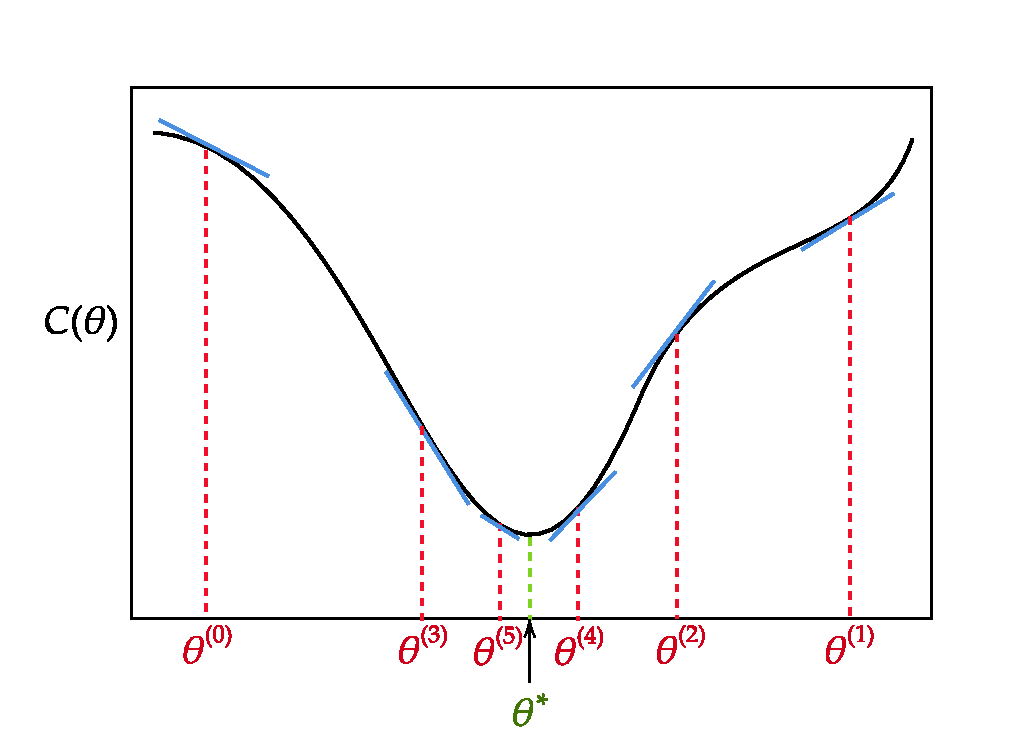
\includegraphics[width=0.99\linewidth, height=0.8\textwidth, trim=20 20 20 20]{figures/GD_1d.pdf}
    \caption{} 
    \vspace{2ex}
  \end{subfigure}%% 
  ~
  \begin{subfigure}[b]{0.5\linewidth}
    \centering
    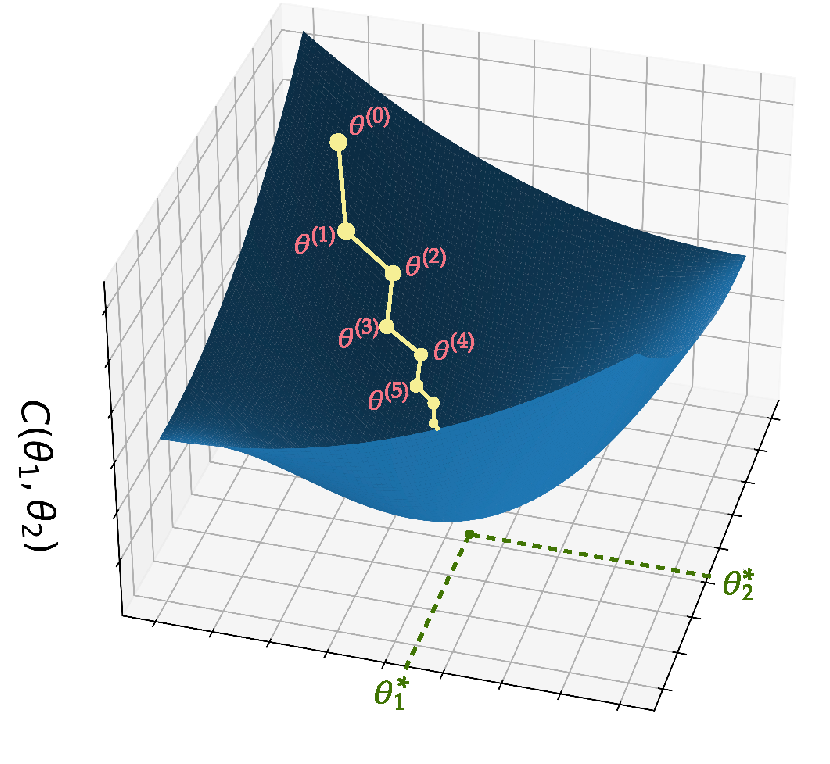
\includegraphics[width=0.9\linewidth, trim=20 20 20 20]{figures/GD_2d.pdf}
    \caption{} 
    \vspace{2ex}
  \end{subfigure} 
    \caption{Illustration of gradient descent for 5 iterations starting with $\theta^{(0)}$ and getting near the optimum $\theta^*$ with $\theta^{(5)}$. (a)~A one-dimensional loss landscape $C(\theta)$ with $\theta \in \mathbb{R}$. (b)~a two-dimensional loss landscape $C(\theta_1,\theta_2)$ with $\theta = (\theta_1, \theta_2) \in \mathbb{R}^2$.}
    \label{simpleloss}
\end{figure}

As an illustration of gradient descent, see Figure~\ref{simpleloss}. First in (a) we consider a  model with a single parameter $\theta \in \mathbb{R}$ and the associated loss function $C(\theta)$ plotted with a minimum at $\theta^*$.  The gradient descent algorithm starts with an initial guess $\theta^{(0)}$ and then updates to $\theta^{(1)}$ using $\theta^{(1)} = \theta^{(0)} - \alpha \nabla C(\theta^{(0)})$. In this simple one dimensional case, the gradient at the point $\theta^{(0)}$ reduces to the derivative, $C'(\theta_0)$, which is the slope of the tangent at the point $\theta^{(0)}$. In our example this derivative is negative, then by multiplying this derivative by $-\alpha$ we move in the opposite direction (right) than the gradient. Using the same process, the next move is driven by $\theta^{(2)} = \theta^{(1)} - \alpha  C'(\theta^{(1)})$. Note that in this case the slope of the tangent at the point $\theta^{(1)}$ is positive. Then by multiplying by $- \alpha $, we are move left towards the minimum. In the figure we show the iterates up to $\theta^{(5)}$ which is not far from the minimal point $\theta^*$.

In Figure~\ref{simpleloss}~(b) we see a similar trajectory, only this time moving on the $(\theta_1, \theta_2)$ plane, and the points are plotted on the surface as $C(\theta^{(i)})$. Here in this example, small steps move in the direction of steepest descent, ultimately reaching a point close to the optimum $\theta^* = (\theta_1^*, \theta_2^*)$. The reader should comprehend that with realistic problems, the number of parameters $d$ can be in the order of millions. Hence each gradient descent iteration is a step in such a high dimensional space, which we cannot visualize. 


%%%%%%%%%%%%%%%%%%%%%%%%%%%%%%%%%%%%%%%%
%%%%%%%%%%%%%%%%%%%%%%%%%%%%%%%%%%%%%%%%
%%%%%%%%%%%%%%%%%%%%%%%%%%%%%%%%%%%%%%%%
\section{Putting Bits Together Into a Deep Neural Network}
\label{sec:putting-bits-together}

Now we are ready to revisit Model~III and fill in a few of the missing details. With deep neural networks, like Model~III, the versatility of the model allows us to in principle approximate any function. In particular, say that in reality we have some unknown function $f^*: \mathbb{R}^p \longrightarrow {\mathbb R}^q$, which is only available to us via data points $(x^{(i)}, y^{(i)})$ with $x^{(i)} \in {\mathbb R}^p$, $y^{(i)} \in {\mathbb R}^q$,  and $y^{(i)} = f^*(x^{(i)})$. If it is a binary classification scenario then $q=1$ and the output can be considered as an element in $[0,1]$. If it is a multi-class classification scenario then $q=K$ and the output can be considered as an element in ${\mathbb R}^K$. If it is a regression problem then again $q=1$ and the output can be any scalar value in ${\mathbb R}$. Finally, in other applications we have vector output ${\mathbb R}^q$ for some $q>1$. In all of these cases, with Model~III we can try and approximate~$f^*(~)$  via the model function \eqref{eq:model-III-f}.

Models I and II are shallow neural networks as they only involve a single layer. As such, they are not able to approximate any arbitrary function very well. However, Model~III when used with multiple layers, is a very rich model, and in principle no matter what $f^*(~)$ we have in reality, with enough training data, and enough computation power for training (gradient descent), we can obtain,
%
\begin{equation}
\label{eq:mod3-approx}
f_{(b^{[1]}, W^{[1]}), \ldots, (b^{[L]}, W^{[L]})} (x) \approx f^*(x).
\end{equation}
%
That is, in general, there exist some parameters ${(b^{[1]}, W^{[1]}), \ldots, (b^{[L]}, W^{[L]})}$ that will enable our model to approximate any function $f^*(~)$. See chapter~5 of \cite{LiquetMokaNazarathy2024DeepLearning} for further discussion about the expressivity of deep neural networks. Let us now dive into a few more details of Model~III.

Recall from  \eqref{eq:dense-layer} that every layer $\ell$ of the model is of the form $f^{[\ell]}(u) = S^{[\ell]}(b^{[\ell]} + W^{[\ell]} u)$ and the model consists of a composition of such layers via \eqref{eq:generalRecursiveModel}. We have already encountered an affine operation similar to $b^{[\ell]} + W^{[\ell]} u$ in the context of Model~II where it was $b + Wx$. Like Model~II we sometimes use a softmax for $S^{[\ell]}(~)$ in the last layer, $\ell=L$, especially when our goal is multi-class classification. Yet for inner layers, $\ell = 1,\ldots,L-1$, we use a (scalar) activation function $\sigma: \mathbb R \to \mathbb R$ and then the structure of the function $S^{[\ell]}(~)$ is via element-wise activations $S^{[\ell]}(z) = \big(\sigma\left(z_{1}\right) ~ \ldots ~\sigma\left(z_{N}\right)\big)$, where $z = (z_1, \ldots, z_N)$. In general, $\sigma(~)$ can be a sigmoid function, as defined in \eqref{eq:first-shallow-view}, or it can be one of other common activation functions in deep learning such as {\em ReLU} or {\em Tanh}; see chapter~5 of \cite{LiquetMokaNazarathy2024DeepLearning} for details. Note that in many texts one just writes, $\sigma(b^{[\ell]} + W^{[\ell]} u)$ for the layer, implying that $\sigma(~)$ is applied element-wise.

We can now revisit Figure~\ref{FFNN} which illustrates a small version of such a model with $L=4$. Observe that for this network,  the input dimension is $p=4$ and the output dimension is $q=1$. The function of each layer $f^{[\ell]}(u) = S^{[\ell]}(b^{[\ell]} + W^{[\ell]} u)$ operates on the outputs of the previous layer (or the input to the network in case $\ell=1$) and yields {\em activation values} (sometimes just called neuron values) of layer $\ell$. We denote these values as $a^{[\ell]}$ and thus for $\ell=1,\ldots,L$,
%
\begin{equation}
\label{eq:s-deep-step}
a^{[\ell]} = f^{[\ell]}(a^{[\ell-1]}),
\qquad
\textrm{where}
\quad
a^{[0]} = x,
\quad
\text{and}
\quad
\hat{y} = a^{[L]}.
\end{equation}
%

What remains to be specified are the dimensions of each of the activations in the network. For example, as the reader may inspect based on the number of neurons (blue nodes) per layer in Figure~\ref{FFNN}, we have that,
%
\begin{equation}
\label{eq:nn-example-dims}
x = a^{[0]} \in {\mathbb R}^4,
\qquad
a^{[1]} \in {\mathbb R}^4,
\qquad
a^{[2]} \in {\mathbb R}^3,
\qquad
a^{[3]} \in {\mathbb R}^5,
\qquad
\hat{y} = a^{[4]} \in {\mathbb R}.
\end{equation}
%
These particular dimensions are part of the specific architecture of the deep neural network and they also imply the dimensions of the model parameters. For example consider layer $\ell=3$ with $f^{[3]}(u) = S^{[3]}(b^{[3]} + W^{[3]} u)$. From \eqref{eq:s-deep-step} we see that $f^{[3]}(~)$ maps $a^{[2]}$ to $a^{[3]}$ and further via \eqref{eq:nn-example-dims} we see that this is a mapping from ${\mathbb R}^3$ to ${\mathbb R}^5$. If we revisit the way that matrix-vector multiplication works as in \eqref{eq:matrix-vector-mult}, we see that we must have $W^{[3]} \in {\mathbb R^{5 \times 3}}$. Further from \eqref{eq:model-ii-vector-add}, we must have $b^{[3]} \in {\mathbb R}^5$. In a similar manner we can consider other layers and see that the dimensions of the individual parameters, $(b^{[1]}, W^{[1]}), \ldots, (b^{[L]}, W^{[L]})$, are specified by the number of activations. The reader may also appreciate that the number of arrows going from layer~2 to layer~3 in Figure~\ref{FFNN} is $15$, exactly matching the $5\times 3=15$ entries of $W^{[\ell]}$. Hence each element in the weight matrix $W^{[\ell]}$ can be considered as an individual {\em weight} on the arrow connecting a neuron from layer $2$ to layer $3$.

As a final illustration, let us unpack the function of the model for the example network from Figure~\ref{FFNN}. When considering the operation at each of the layers one after the other we obtain,

\begin{equation}
\label{eqn:opened-out-example-2}
\hat{y} =S^{[4]}(W^{[4]}S^{[3]}(W^{[3]}S^{[2]}(W^{[2]}S^{[1]}(W^{[1]}x+b^{[1]})+b^{[2]}) +b^{[3]})+b^{[4]}).
\end{equation}
In fact, the reader may work out that the number of parameters is,
%
\begin{equation}
\label{eq:61-is-the-number}
d = \underbrace{4\times4 + 4}_{\text{Hidden layer 1}} + \underbrace{3\times 4 + 3}_{\text{Hidden layer 2}}+ \underbrace{5\times 3 + 5}_{\text{Hidden layer 3}}  + \underbrace{1 \times 5 +1}_{\text{Output layer}}  = 61.
\end{equation}
%
Hence, when training such a model via gradient descent, each time we compute the gradient, we obtain a gradient vector in ${\mathbb R}^{61}$. More realistic models may have many more activations (neurons), and sometimes more layers as well. Hence the number of parameters, $d$, easily climbs to millions or more, and this is why training large deep neural networks may be very expensive in terms of time, hardware, and power.

%%%%%%%%%%%%%%%%%%
%%%%%%%%%%%%%%%%%%%%%%%%%%%%%%%%%%%%%%%%
\section{More Advanced Models}
\label{sec:more-advanced-models}

Deep neural networks have been extended way beyond Model~III, yet the good news is that for more advanced models, generally one does not necessarily need more advanced mathematics. In this section, we present some key mathematical constructs used beyond models I -- III. We present  the {\em convolution} operation used in {\em convolutional neural networks} (CNNs), {\em word embedding} used in sequence models such as {\em recurrent neural network} (RNNs) or {\em long short term memory} (LSTM) models, and the {\em attention mechanism} used in {\em transformer} models that power current state of the art {\em large language models}.

Convolutional neural networks have revolutionized the field of computer vision. Fundamentally, CNNs leverage the concept of the convolution, a mathematical operation that involves applying a {\em filter}, also known as a {\em kernel}, across an input data grid to extract local patterns or features. This process is akin to sliding a window over an image and with each move computing the {\em inner product} between the elements of the (vectorized) kernel and the elements of the corresponding region of the (vectorized) image. The convolution operation between two matrices $W$ and $x$ is denoted as $z = W \star x$. There are different versions of the convolution operation. Here, we present a basic version and for more general scenarios, refer to chapter 6 of  \cite{LiquetMokaNazarathy2024DeepLearning}. To understand this basic version, assume that $x$ is a grayscale image of size $100 \times 100$ and the kernel $W$ is a $3\times 3$ matrix of weight parameters represented as
%
\begin{equation}
\label{eq:conv-kernel}
W = 
\begin{bmatrix}
    w_{1,1} & w_{1,2} & w_{1,3} \\
    w_{2,1} & w_{2,2} & w_{2,3} \\
    w_{3,1} & w_{3,2} & w_{3,3} \\
\end{bmatrix}.
\end{equation}
%
Note that the kernel matrix $W$ is usually much smaller than the image $x$. We slide the kernel over the image to perform the convolution operation. As in the case of Model~III, the best values for the weight parameters ($w_{i, j}$ entries in $W$) are learned during the training process. 

In the basic version for this example, the result $z$ of the convolution operation is a matrix of dimension $(100 - 3 + 1) \times (100 - 3 + 1) = 98 \times 98$ with the $(i, j)$-th element of $z$ computed as 
%
\begin{equation}
\label{eq:conv-explicit}
z_{i,j} = \sum_{i'=0}^{2} \sum_{j'=0}^{2} x_{i+i', j+j'}  \cdot \, w_{i'+1, j'+1}
\qquad
\textrm{for}
\qquad i, j \in \{1, \dots, 98\}.
\end{equation}
%
Here \( x_{i+i', j+j'} \) represents the pixel value at position \( (i+i', j+j') \) in the input image, and \( w_{i'+1, j'+1} \) represents the weight parameter at position \( (i'+1, j'+1) \) in the kernel. For instance, to compute the value $z_{1, 1}$,% on the output feature map $z$, 
we perform the calculation,
%
\begin{equation}
\label{eq:very-spcific-conv}
z_{1,1} = \sum_{i'=0}^{2} \sum_{j'=0}^{2} x_{1+i', 1+j'} \cdot w_{i'+1, j'+1}.
\end{equation}
%
Note that $z_{1,1}$ is the result of an inner product between the vectorized $W$ and the vectorized $3\times 3$ top-left submatrix of $x$. 

Similarly, we compute all the elements of $z$ by sliding the kernel over the image and performing such an inner product each time between the kernel $W$ and the corresponding submatrix of $x$. After performing the convolution operation between the image and the kernel, a convolutional layer in a CNN applies an activation function, just like in Model~III. This yields what is sometimes called a {\em feature map} that highlights certain patterns or features present in the image. Now just like in Model~III, the feature map serves as input to subsequent layers in the CNN for further processing and analysis.

It's important to note that CNNs involve other operations, such as pooling, and various architectural configurations including multiple channels (feature maps) per layer, skip connections, integration of fully connected layers, and others. See chapter~6 of \cite{LiquetMokaNazarathy2024DeepLearning} for more details. We also note that from an historical perspective, the work in \cite{krizhevsky2012imagenetxxxqqq} was pivotal in highlighting the strength of deep learning, and convolutional neural networks in particular.

While CNNs are excellent for tasks like image recognition, sequential data such as text, often requires a different approach. This is where sequence models like recurrent neural networks (RNNs) and long short term memory (LSTM) models come into play. Unlike CNNs which process the entire input at once, RNNs and LSTMs process the data sequentially one element at a time. In doing so, these models maintain an internal state that captures information about previous elements in the sequence.

One key challenge in using RNNs and LSTMs for natural language processing tasks is how to represent words as numerical vectors such that these models can understand the data. This is where {\em word embedding} becomes useful. Word embedding is a technique used to represent words as vectors, where the vectors corresponding to similar words, remain close to each other. Via the vector representation of the words, similarity between any two words is measured by the cosine of the angle between the corresponding two vectors using formula~\eqref{eq:cosine-angle-vec}.  

For example, the word \texttt{king} could be represented by the vector $(0.41, \, 1.2,\, 3.4, \,-1.3)$ and the word \texttt{queen} can be represented by a relatively similar vector such as $(0.39, \, 1.1, \, 3.5, \, 1.6)$. Then a completely different word such as \texttt{mean} might be represented by a vector such as $(-0.2,\, -3.2,\, 1.3,\, 0.8)$. One can now verify in this example, that the cosine of the angle between the words \texttt{king} and \texttt{queen} is about $0.729$ while the cosine of the angle between \texttt{mean} and the other two words is lower, which is at about $-0.04$ for \texttt{king} and $0.156$ for \texttt{queen}, respectively. 

With such a word embedding approach, the typical way we process input text is to convert each word (or sometimes a similar notion known as a {\em token}) to a vector. Hence the input to a model, is not just a single vector $x$ as is the case for models I --- III, but is rather a sequence of vectors. Then an RNN model or LSTM model processes this sequence, one by one, keeping an internal state and also resulting in an output sequence. This technique has proven valuable for many language tasks including translation among others. For a description of how classical models such as RNN models or LSTM models deal with such data,  see chapter~7 of \cite{LiquetMokaNazarathy2024DeepLearning}.

Recurrent neural networks, long short term memory models, and a few variants were the main sequence models in deep learning up to recent times. However, in the last few years, following the 2017 paper \cite{vaswani2017attention}, a completely different approach, called {\em transformer} models has emerged and is now the main tool used in contemporary large language models. Transformers overcome, limitations of RNNs and LSTM models, such as difficulty in parallelization and difficulty in capturing long-range dependencies (even though LSTM models are explicitly designed for enabling long range memory). Transformers address these limitations, primarily by leveraging on an idea called the {\em attention mechanism}. Unlike RNNs and LSTMs, which process inputs sequentially, transformers process all words simultaneously, enabling highly efficient parallel computation. This parallelization makes transformers particularly well-suited for handling long sequences, such as those encountered in machine translation, document summarization tasks, and general interactions with large language models via chat. While we leave a complete description of the transformers architecture to  chapter~7 of \cite{LiquetMokaNazarathy2024DeepLearning}, or other sources, let us see now how basics of the attention mechanism can be described via inner products and the softmax function.

When processing each word, the attention mechanism allows the model to focus on relevant parts of the input sequence. That is, by ``attending'' from each word to every other word, we capture dependencies across the entire sequence. Imagine reading a long piece of text and trying to summarize it. Instead of reading the entire text from start to finish every time, one can generate a summary by focusing on the most relevant parts, or key words. This selective focus is analogous to what the attention mechanism does. At a high level, we assign a weight to each input word based on its relevance to the current word being processed. This weight determines how much attention the model should pay to that input word when generating the output associated with the current word. 

Mathematically, to understand the attention mechanism, consider a sequence of words $x^{{\langle 1 \rangle}},\ldots, x^{{\langle T \rangle}}$ where each $x^{{\langle t \rangle}}$ is a vector representing a word (or token) using our word embedding scheme. Our goal is to compute the attention weights for a specific current word, $x^{{\langle t \rangle}}$. %, in the sequence. 
We begin by calculating a {\em score} (also called {\em alignment score}) for all other input words, $x^{{\langle j \rangle}}$,  based on their similarity to $x^{{\langle t \rangle}}$. A basic form for such an alignment score is using the inner product,
%
\begin{equation}
\label{eq:score}
s(x^{{\langle t \rangle}},x^{{\langle j \rangle}})=(x^{{\langle t \rangle}})^\top x^{{\langle j \rangle}}.% \qquad 
%j = 1,\ldots,T.
\end{equation}

These scores, computed for $j = 1,\ldots,T$, are then passed through the softmax function, $S_{\text{softmax}}(~)$, defined in \eqref{eq:softeq}, which squashes them into a probability vector $(\alpha_1, \ldots, \alpha_T)$. Namely the attention weight of any input word $j$ from the perspective of the current word $t$ is,
%
\begin{equation}
\label{eq:attentionweight}
\alpha_{j} = \frac{e^{s(x^{{\langle t \rangle}},x^{{\langle j \rangle}})}}{\sum_{t'=1}^T e^{s(x^{{\langle t \rangle}},x^{{\langle t' \rangle}})}}.
\end{equation}
%

The probability vector $(\alpha_1, \ldots, \alpha_T)$ represents how much attention each input word $x^{{\langle j \rangle}}$ should receive when we handle the current word $x^{{\langle t \rangle}}$. Intuitively, due to the inner product operation used in \eqref{eq:score}, input words that are more similar to the current word will have higher attention weights, indicating that they are more relevant for generating the output. Conversely, input words that are less relevant will have lower attention weights, meaning they contribute less to the output generation process. By selectively attending to the most relevant parts of the input sequence, the attention mechanism enables us to capture long-range dependencies and learn complex patterns in the data. This yields a setup that is highly effective for a wide range of natural language processing tasks, from language translation to text generation.

%%%%%%%%%%%%%%%%%%%%%%%%%%%%%%%%%%%%%%%%
%%%%%%%%%%%%%%%%%%%%%%%%%%%%%%%%%%%%%%%%
%%%%%%%%%%%%%%%%%%%%%%%%%%%%%%%%%%%%%%%%
\section{Conclusion and Outlook}
\label{sec:conclusion}

While our ultimate goal is deep learning, our focus in this document was mathematical background. For this we covered many elementary components of mathematical notation used in conveying deep learning ideas. Such a survey cannot replace solid mathematical foundations, yet we hope that it enables scientists that do not often use mathematics, to engage with mathematical descriptions of deep learning models and algorithms. We can also consider the presentation here as a gentle introduction (or review) for readers wanting to study our book, {\em Mathematical Engineering of Deep Learning} \cite{LiquetMokaNazarathy2024DeepLearning}, as well as the other books we mentioned at the introduction. While the presentation here does not empower the reader with all of the needed mathematical background, it does enable the reader to follow a solid portion of the content from such a book. Readers wishing to further strengthen their foundations are encouraged to follow standard courses and books in calculus, linear algebra, probability, and statistics.\footnotemark{}

\footnotetext{See \url{https://deeplearningmath.org/} for specific suggestions.}

This is a summary of the key mathematical content that we covered. We covered sets and their elements, as well as summation notation with sets. We covered basic set notation for the real numbers ${\mathbb R}$ as well as notation for vectors ${\mathbb R}^n$, and matrices ${\mathbb R}^{m \times n}$. We covered declaration of functions using notation such as $f: {\cal A} \to {\cal B}$, where ${\cal A}$ and ${\cal B}$ are sets. We covered basics of vectors, but without their geometric interpretation, a topic that the reader can pick up elsewhere. In particular we covered inner products, Euclidean norms, cosine of the angle, the Euclidean distance between vectors, and mean squared error. We also covered basics of matrices including elementary definitions, diagonal matrices, symmetric matrices, identity matrices, matrix transpose, and importantly matrix multiplication (including matrix-vector multiplication). We also mentioned element-wise operations on vectors and matrices, matrix inverses, and tensors. Finally we covered gradient vectors, the key component for gradient descent learning (optimization). As we saw, this dense manifest of ``basic mathematical knowledge'' can go a long way in helping to describe complex deep learning models, and we revisited our Models I -- III throughout, connecting the basic notation of these models to the elementary mathematical principles.

In terms of models beyond our example models I -- III, we briefly highlighted ideas of convolutions, word embedding, and the attention mechanism. Other aspects of deep learning that we did not cover include generative models such as generative adversarial networks, variational autoencoders, diffusion models, reinforcement learning, and graph neural networks. Admittedly, some of these concepts may require more mathematical background than we provided here. The reader may see chapter~8 of \cite{LiquetMokaNazarathy2024DeepLearning} for an overview of this assortment of topics. 

\bibliographystyle{apalike}
\bibliography{BibForTheDLBook.bib}

\end{document}
